\documentclass[11pt,a4paper]{article}

\usepackage[utf8]{inputenc}
\usepackage[margin=2.5cm]{geometry}
\usepackage{amsmath,amssymb}
\usepackage{graphicx}
\usepackage{booktabs,multirow,makecell,tabularx,threeparttable}
\usepackage{caption,subcaption}
\usepackage{enumitem}
\usepackage{xcolor}
\usepackage{tikz}
\usetikzlibrary{positioning,arrows.meta,fit,backgrounds,calc}
\usepackage{fancyhdr}
\usepackage{microtype}
\usepackage{float}
\usepackage{afterpage}
\makeatletter\setlength{\@fptop}{0pt}\setlength{\@fpbot}{0pt plus 1fil}\makeatother
\usepackage[hidelinks]{hyperref}
\usepackage[numbers,sort&compress]{natbib}
\newcommand{\seerLeakAUC}{0.735}
\newcommand{\seerLeakSD}{0.031}
\newcommand{\seerLeakCI}{0.701--0.768}
\newcommand{\seerLeakBE}{0.131 / 0.149}
\newcommand{\seerLeakECE}{0.149}
\newcommand{\seerPCAAUC}{0.735}
\newcommand{\seerPCASD}{0.031}
\newcommand{\seerPCACI}{0.701--0.768}
\newcommand{\seerPCABE}{0.131 / 0.149}
\newcommand{\seerPCAECE}{0.149}
\newcommand{\seerRFAUC}{0.741}
\newcommand{\seerRFSD}{0.027}
\newcommand{\seerRFCI}{0.713--0.770}
\newcommand{\seerRFBE}{0.130 / 0.146}
\newcommand{\seerRFECE}{0.146}
\newcommand{\seerUniAUC}{0.739}
\newcommand{\seerUniSD}{0.028}
\newcommand{\seerUniCI}{95\% CI 0.709--0.769}
\newcommand{\seerUniBE}{0.130 / 0.146}
\newcommand{\seerUniECE}{0.146}
\newcommand{\seerUniCIs}{0.709--0.769}
\newcommand{\seerUniP}{0.5607}
\newcommand{\seerUniTOST}{0.2251}
\newcommand{\seerCITL}{$-$1.00}
\newcommand{\seerSlope}{1.17}
\newcommand{\seerMeanPred}{28.6}
\newcommand{\seerDiffUL}{+0.0043}
\newcommand{\seerDiffULci}{$-$0.0082 to +0.0169}
\newcommand{\seerDiffPL}{+0.0000}
\newcommand{\seerDiffPLci}{$-$0.0014 to +0.0014}
\newcommand{\seerConfCov}{95.26}
\newcommand{\seerConfSingle}{61.92}
\newcommand{\seerConfAmb}{38.08}
\newcommand{\seerNcal}{556}
\newcommand{\seerNcalEv}{78}
\newcommand{\seerLbAcc}{83.50}
\newcommand{\seerLbAccCI}{79.96--86.52}
\newcommand{\seerLbBal}{63.73}
\newcommand{\seerLbSens}{36.23\% (25/69)}
\newcommand{\seerLbSpec}{91.23\% (385/422)}
\newcommand{\seerLbAUC}{0.722}
\newcommand{\seerLbAUCCI}{0.646--0.790}
\newcommand{\seerLbBrier}{0.132}
\newcommand{\seerLbBrierCI}{0.121--0.144}
\newcommand{\seerLbSlope}{1.03}
\newcommand{\seerLbSlopeCI}{0.69 to 1.41}
\newcommand{\seerLbInt}{$-$1.00}
\newcommand{\seerLbIntCI}{$-$1.22 to $-$0.78}
\newcommand{\seerLbCITL}{$-$1.02}
\newcommand{\seerLbCITLCI}{$-$1.10 to $-$0.94}
\newcommand{\seerLbCov}{95.32}
\newcommand{\seerLbCovCI}{93.07--96.86}
\newcommand{\wbcdLbBrier}{0.010}
\newcommand{\wbcdLbBrierCI}{0.004--0.017}
\newcommand{\seerRFfolds}{31}
\newcommand{\seerRFpct}{89}
\newcommand{\seerShapTop}{progesterone receptor status, N stage, number of positive regional nodes, age and histological grade}
\newcommand{\seerDCAlo}{0.09}
\newcommand{\seerDCAhi}{0.16}
\newcommand{\seerCovRange}{94.0\% to 96.5\%}
\newcommand{\seerMaxSMD}{$\le$0.08}
\newcommand{\seerNcompRange}{maximal fluctuation 0.0527 AUROC}
\newcommand{\seerFairText}{Discrimination was similar across racial groups (AUROC 0.738 White, 0.729 Black, 0.765 Other; overlapping CIs) but declined with age (0.774 for $<$50 years vs 0.699 for 60--69 years). Calibration differed markedly: the model overpredicted risk in all groups, but least for Black patients (CITL $-$0.40, 95\% CI $-$0.51 to $-$0.28; observed risk 24.4\% vs predicted 31.4\%) and most for Other-race patients (CITL $-$1.44; observed 8.6\% vs predicted 26.3\%). Because predicted risks varied much less between groups than observed risks, the model compressed the higher mortality of Black patients relative to other groups, so a single recalibration would not correct all groups equally. Sensitivity at the 0.5 threshold was lowest for Other-race (22.2\%) and Black (25.5\%) patients, and conformal coverage ranged from 94.0\% to 96.5\%. Subgroup sizes, particularly the 51 events among Black and 18 among Other-race patients, make these estimates imprecise.}

\makeatletter\newcommand{\inputrows}[1]{\@@input #1 }\makeatother

\captionsetup{font=small,labelfont=bf}
\pagestyle{fancy}\fancyhf{}
\lhead{\small\itshape TRUST-BC: Multicohort Benchmark}\rhead{\small\thepage}
\renewcommand{\headrulewidth}{0.4pt}
\setlength{\parskip}{3pt}
\setlist{itemsep=2pt,topsep=3pt}
\renewcommand{\labelitemi}{$\bullet$}

\title{\textbf{TRUST-BC: A Multicohort Benchmark for Leakage-Free, Calibrated, and Uncertainty-Aware Breast Cancer Prediction Models}}
\author{Mohammad Amin Shayegan\textsuperscript{1,*}, Reza Abolghasemi\textsuperscript{1,*},\\ Mohammadreza Salehi\textsuperscript{1}, Armaghan Kiarsi\textsuperscript{2}\\[6pt]
\small\textsuperscript{1}Department of Computer, Shi.C., Islamic Azad University, Shiraz, Iran\\
\small\textsuperscript{2}Faculty of Health, Medicine and Society (Oncology), University of Chester, Chester, United Kingdom\\
\small\textsuperscript{*}Corresponding authors: MA.Shayegan@iau.ac.ir; Reza.Abolghasemi@iau.ir}
\date{}

\renewcommand{\cellalign}{lc}\renewcommand{\theadalign}{lc}
\newcolumntype{P}[1]{>{\raggedright\arraybackslash\hspace{0pt}}p{#1}}
\newcolumntype{Y}{>{\raggedright\arraybackslash\hspace{0pt}}X}
\begin{document}
\maketitle\thispagestyle{fancy}

\begin{abstract}\label{sec:abstract}
\noindent\textbf{Background:} Machine learning models for breast cancer prediction frequently report accuracies above 97\%, yet preprocessing leakage, miscalibration, and mishandled censoring can distort these estimates and impede clinical translation.

\noindent\textbf{Methods:} We developed TRUST-BC, an open-source benchmark applied to three public cohorts: the Wisconsin Diagnostic Breast Cancer dataset ($n=569$), the Coimbra biomarker cohort ($n=116$), and a SEER registry extraction ($N=4{,}024$; 3,270 patients with 458 deaths in the 5-year classification cohort). The framework combines leakage-free repeated nested cross-validation, an architecture-matched leaky comparator, Nadeau--Bengio corrected inference with equivalence testing, calibration and decision curve analysis, split conformal prediction, subgroup analysis, and a penalised Weibull survival model. Models were evaluated once on a 15\% held-out partition.

\noindent\textbf{Results:} Cross-validated accuracy was 97.08\% (95\% CI 95.34--98.82) for WBCD and 71.35\% (62.27--80.43) for Coimbra, and the SEER AUROC was \seerUniAUC{} (\seerUniCIs). Global scaling and PCA leakage changed performance by at most 0.52 percentage points or 0.001 AUROC. SEER probabilities were systematically overestimated (calibration-in-the-large \seerCITL), and conformal coverage was \seerConfCov\% overall but 69.9\% among patients who died. The survival model achieved a C-index of 0.722 (95\% CI 0.675--0.771).

\noindent\textbf{Conclusions:} Leakage, calibration, and predictive uncertainty behaved differently across cohorts and should be audited per dataset rather than assumed. TRUST-BC provides a reusable template, reported following TRIPOD+AI, for this purpose.

\medskip
\noindent\textbf{Keywords:} Breast Cancer; Machine Learning; Data Leakage; Conformal Prediction; Probability Calibration; TRIPOD+AI.
\end{abstract}

\section{Introduction}\label{sec:introduction}
\subsection{Clinical Motivation and Computational Pitfalls in Oncology Modeling}\label{sec:clinical-motivation-and-comput}
In 2022, breast cancer was the most commonly diagnosed cancer and the leading cause of cancer death among women worldwide, with an estimated 2.3 million new cases and approximately 670,000 deaths~\cite{bray2024}. Accurate early diagnosis and long-term prognostic risk assessment are essential for the design of standard treatments, including surgical resection, systemic adjuvant chemotherapy, and targeted endocrine therapies. Over the past decade, high discriminative performance has been achieved by supervised machine learning (ML) models (support vector machines, tree ensembles, and gradient boosting architectures~\cite{xgboost,lightgbm}) on retrospective tabular oncology benchmarks.

Despite these promising benchmark metrics, translation into clinical practice remains challenging~\cite{kubiak2025}. Widespread methodological vulnerabilities impair reproducibility and translational validity across the biomedical ML literature~\cite{kapoor2023}. Four structural vulnerabilities are particularly common in clinical oncology workflows~\cite{collins2025onc}:
\begin{itemize}
\item \textbf{Parametric and covariance data leakage:} preprocessing transforms such as standard scaling and principal component analysis (PCA) are often fit on the entire dataset before splitting. Even if sample identifiers do not overlap between splits, global distributional statistics leak across folds and may produce optimistic performance estimates.
\item \textbf{Probability miscalibration:} optimisation objectives focus on discrimination (accuracy, AUROC) and neglect calibration~\cite{vancalster2016,steyerberg2019}, so predicted probabilities often do not match observed event rates.
\item \textbf{Censoring and horizon misclassification in registries:} when time-to-event cohorts are converted into fixed-horizon binary targets, patients censored before the horizon are often labelled as non-events, and deaths occurring after the horizon are often labelled as events, both producing systematic label error.
\item \textbf{Lack of clinical uncertainty quantification:} classifiers yield point probabilities without distribution-free coverage guarantees, leaving clinicians without safety filters for borderline or atypical presentations~\cite{vazquez2022}.
\end{itemize}

The three cohorts studied here correspond to different prediction tasks. WBCD and Coimbra are \emph{diagnostic} settings, in which the model estimates whether breast cancer is present at the time of sampling (from fine-needle aspirate cytology and from routine serum biomarkers, respectively). SEER is a \emph{prognostic} setting, in which the model estimates the risk of death from any cause within 5 years of diagnosis. The intended users of such models are clinicians (cytopathologists, breast surgeons and oncologists) using them as decision support, not patients or autonomous systems. In this study the models serve primarily as test cases for the auditing template rather than as candidates for immediate deployment.

\subsection{Related Work and Methodological Deficits in Current Literature}\label{sec:related-work-and-methodologica}
Machine learning algorithms have been applied to tabular breast cancer cohorts with varying methodological rigour. On the morphological WBCD benchmark, reported accuracies often exceed 97\%, but unsupervised feature transforms seldom occur within cross-validation loops, with the potential for covariance leakage. Models evaluating multi-biomarker panels on serum metabolic profiles (Coimbra cohort) have often relied on unnested or uncalibrated splits~\cite{patricio2018}. Studies of population-scale cancer registries such as SEER frequently transform follow-up records into 5-year survival targets without accounting for patients censored before 60 months, distorting the ground-truth outcome distribution.

Recent prognostic studies, including the comparative re-analysis benchmark by Tadj et al. (2026)~\cite{tadj2026}, show increasing interest in systematic evaluation, but many studies still rely on heuristic shortcuts. First, cross-validation fold scores are commonly compared using paired $t$-tests without correcting for the positive correlation induced by overlapping training sets, which inflates the Type I error rate~\cite{nadeau2003}. For single-split comparisons on a fixed test set, DeLong's test provides a valid nonparametric comparison of correlated AUROCs~\cite{delong1988}, but it does not resolve the fold-correlation problem across repeated cross-validation. Second, models often produce point probabilities with no uncertainty intervals or triage mechanisms. Third, sensitivity to sample size and feature-subspace dimensionality is largely unquantified. Table~\ref{tab:lit} (Section~\ref{sec:disc}) compares existing literature with the safeguards used in this work.

This disconnect is not unique to oncology. A systematic review and meta-analysis of 21 cardiovascular ML studies using electronic health records reported substantial heterogeneity ($I^2>99\%$) and potential publication bias, concluding that methodological concerns currently limit clinical applicability~\cite{liu2025}. Cai et al.~\cite{cai2024} identified recurrent cardiovascular ML pitfalls involving data quality, small samples and low event rates, overfitting, inadequate evaluation criteria, and limited generalisability, and recommended separating training, tuning and testing data. These observations indicate that the vulnerabilities addressed by TRUST-BC are part of a systemic pattern across clinical ML, supporting the need for a reusable auditing template.

Breast cancer outcomes also differ across sociodemographic groups. In the United States, Black women have higher breast cancer mortality than White women despite similar or lower incidence, and differences in stage at diagnosis, tumour subtype and access to treatment have been described across racial, age and socioeconomic groups~\cite{acs2024}. Prediction models developed on registry data can reproduce or amplify such differences if performance or calibration varies between groups; TRIPOD+AI therefore recommends reporting performance in key sociodemographic subgroups~\cite{collins2024tripod}, which we do for race and age in the SEER cohort.

\subsection{Objectives and Key Contributions}\label{sec:objectives-and-key-contributio}
Unlike prior single-cohort leakage audits~\cite{tadj2026} that addressed pre-split oversampling contamination and temporal misalignment within a single registry, this work presents TRUST-BC, an open-source auditing and modelling template that concurrently addresses parametric leakage, horizon- and censoring-driven label error, probability miscalibration, and the lack of distribution-free uncertainty quantification across three different data archetypes (cytopathological, metabolic, and epidemiological registry). Methodologically, this is a model development study with internal validation (repeated nested cross-validation and a single held-out partition from the same data source); no external validation was performed.

This study makes six methodological contributions:
\begin{enumerate}
\item \textbf{Parametric isolation by construction:} feature standardisation, dimensional reduction and hyperparameter tuning are encapsulated in the inner cross-validation folds through scikit-learn pipelines~\cite{sklearn}.
\item \textbf{Equivalence and superiority testing:} model differences are evaluated with the Nadeau--Bengio corrected resampled $t$-test~\cite{nadeau2003} with Holm--Bonferroni control~\cite{holm1979}, combined with Two One-Sided Tests (TOST)~\cite{schuirmann1987,walker2011} with pre-specified margins ($\Delta=0.02$ for accuracy, $\Delta=0.01$ for AUROC), and complemented by an architecture-matched leakage contrast.
\item \textbf{Finite-sample uncertainty quantification:} inductive split conformal prediction~\cite{angelopoulos2021,vovk2005} generates prediction sets with a marginal coverage guarantee ($1-\alpha=95\%$) and flags ambiguous cases for expert review.
\item \textbf{Calibration assessment and decision analysis:} Brier score, expected calibration error (ECE)~\cite{vancalster2019}, calibration slope, intercept and calibration-in-the-large, and decision curve analysis (DCA)~\cite{vickers2006}.
\item \textbf{Fixed-horizon registry labelling and survival modelling:} for the SEER cohort, patients with unknown 5-year status are excluded and deaths after month 60 are labelled as 5-year survivors, and a penalised Weibull accelerated failure time (AFT) model with Kaplan--Meier risk stratification is used for continuous time-to-event prediction.
\item \textbf{Transparent reporting:} the study is reported following TRIPOD+AI~\cite{collins2024tripod}. Design choices were informed by the domains of PROBAST+AI~\cite{moons2025probast}, and an author self-assessment against PROBAST+AI is provided in the Supplementary Material for transparency; it is not a substitute for independent appraisal.
\end{enumerate}

We bundle these components into one template because in practice these vulnerabilities co-occur and interact: a model tuned to eliminate leakage but not audited for calibration and uncertainty can create a false sense of methodological rigour. The contribution of TRUST-BC is this joint auditing capability rather than any individual component. Leakage-aware and calibration-aware evaluation frameworks have been proposed for other clinical tabular domains, but these typically address a single vulnerability in a single cohort. The principal contribution of TRUST-BC is therefore methodological rather than a claim of superior empirical prediction: it integrates six independently established but rarely co-implemented safeguards into a single reusable pipeline. TRUST-BC is intended primarily as a public auditing framework rather than as a single deployable predictive model.


\section{Materials and Methods}\label{sec:materials-and-methods}
\subsection{Cohort Descriptions, Setting, and Sample Size}\label{sec:cohort-descriptions-setting-an}
We evaluated the framework on three cohorts representing distinct diagnostic and prognostic contexts (Table~\ref{tab:cohorts}). Participant flow is shown in Supplementary Figure~S1 and participant characteristics by partition in Supplementary Table~S3.

\begin{table}[htbp]
\centering\small
\caption{Cohort characteristics, outcome distributions, and deterministic partitions.}\label{tab:cohorts}
\setlength{\tabcolsep}{4pt}
\begin{tabularx}{\textwidth}{@{}P{1.5cm}P{0.9cm}P{0.5cm}YP{2.6cm}P{1.9cm}P{1.9cm}@{}}
\toprule
\textbf{Cohort} & \textbf{$N$} & \textbf{$D$} & \textbf{Clinical endpoint} & \textbf{Class distribution} & \textbf{Development set (85\%)} & \textbf{Lockbox (15\%)}\\
\midrule
WBCD & 569 & 30 & FNA malignancy & 357 benign / 212 malignant & 483 (180 events) & 86 (32 events)\\
Coimbra & 116 & 9 & Breast cancer status (case--control) & 52 controls / 64 cases & 98 (54 events) & 18 (10 events)\\
SEER (5-year) & 3,270 & 16 & All-cause death within 60 months & 2,812 alive at 60 months / 458 deaths & 2,779 (389 events) & 491 (69 events)\\
SEER (survival) & 4,024 & 16 & Time to all-cause death & 3,408 censored / 616 deaths & 3,219, 80\% (493 events) & 805, 20\% (123 events)\\
\bottomrule
\end{tabularx}
\end{table}

\begin{itemize}
\item \textbf{Wisconsin Diagnostic Breast Cancer (WBCD):} $n=569$ fine-needle aspirate (FNA) samples (357 benign, 212 malignant) from patients with breast masses at a single centre (University of Wisconsin Hospitals, Madison, WI, USA), collected before 1993 and distributed through the UCI Machine Learning Repository~\cite{street1993,uci}. Thirty real-valued features describe nuclear morphology (mean, standard error, and worst value of ten characteristics) computed from digitised images after an operator initialised the nuclear boundaries, so predictor measurement contains a subjective component~\cite{street1993}; operator characteristics are not reported in the source. Diagnoses were those established by the source investigators~\cite{street1993}. The dataset contains no missing values. With 212 events and 30 candidate predictors, the events-per-variable (EPV) ratio is 7.1.
\item \textbf{Coimbra biomarker cohort:} $n=116$ women (64 with newly diagnosed breast cancer before any treatment and 52 healthy controls) recruited at the Gynaecology Department of the University Hospital Centre of Coimbra, Portugal (single centre) between 2009 and 2013~\cite{patricio2018}. Nine routine clinical and metabolic predictors (age, body mass index [BMI], glucose, insulin, homeostatic model assessment of insulin resistance [HOMA-IR], leptin, adiponectin, resistin, and monocyte chemoattractant protein-1 [MCP-1]) were measured from fasting blood samples collected at the first consultation~\cite{patricio2018,uci}. The design is case--control; because a case--control sample does not reflect the case mix or prevalence of a screening population, predicted probabilities and calibration in this cohort are not transferable to screening. The dataset contains no missing values. The EPV, computed from the smaller outcome class (52 controls), is 5.8, below conventional heuristics; this cohort is therefore analysed as a small-sample stress test of the framework rather than as a basis for a deployable model.
\item \textbf{SEER registry research benchmark:} a curated public extraction of the National Cancer Institute (NCI) Surveillance, Epidemiology, and End Results (SEER) program~\cite{namdari2019,seer2026}: $N=4{,}024$ female patients with infiltrating ductal or lobular carcinoma (histology code 8522/3) diagnosed between 2006 and 2010, extracted from the November 2017 submission after excluding cases with unknown tumour size, unexamined regional lymph nodes, or survival under one month~\cite{namdari2019,amartey2024}. SEER is a population-based network of US cancer registries; registry identifiers are not included in the extraction, so heterogeneity across registries could not be examined. In the analysed file, all patients were aged 30--69 years and all had positive regional nodes (N1--N3), which restricts the population to which the results apply. Follow-up extended to a maximum of 107 months (median 73). We cross-checked the total cohort size ($N=4{,}024$) and the 616 deaths against the dataset record. The classification cohort includes 12 raw clinical and demographic predictors, giving 16 numeric features after one-hot encoding of race, marital status, A stage, and estrogen and progesterone receptor status. With 458 events within 60 months, the raw-predictor EPV is 38.2 and the model-input EPV is 28.6. The observed 60-month all-cause mortality of 14.0\% (458/3,270) should not be interpreted as 1 minus population-level relative survival (about 91\% at 5 years~\cite{acs2024}), because relative survival adjusts for expected background mortality and this cohort is restricted to node-positive disease. We did not have access to re-derive this extraction through SEER*Stat; the public file is therefore used for methodological benchmarking rather than clinical deployment.
\end{itemize}

Treatment information (surgery, radiotherapy, chemotherapy, endocrine and anti-HER2 therapy) was not available in the SEER extraction and was not used as a predictor, so predicted 5-year mortality should be interpreted as risk under the treatments received by the 2006--2010 cohort. Treatment is not relevant to the diagnostic cohorts, in which samples were obtained before treatment.

\paragraph{Predictors.} All available predictors in each dataset were considered as candidates, with the exception of the composite stage variable in SEER (6th-edition AJCC stage), which was excluded to avoid collinearity with its components. Ordinal staging descriptors were integer coded:
\begin{equation}
\text{T} \in \{\text{T1}{:}1,\text{T2}{:}2,\text{T3}{:}3,\text{T4}{:}4\},\quad
\text{N} \in \{\text{N1}{:}1,\text{N2}{:}2,\text{N3}{:}3\},\quad
\text{Grade} \in \{\text{I}{:}1,\text{II}{:}2,\text{III}{:}3,\text{IV}{:}4\}.
\end{equation}
Such coding assumes linear spacing among ordinal categories; alternative representations were not benchmarked. SEER predictors were abstracted by certified tumour registrars at diagnosis.

\paragraph{Sample size.} No a priori sample size calculation was possible because all datasets were fixed public cohorts. The EPV heuristic~\cite{steyerberg2019} was developed for unpenalised logistic regression and is reported only as a conventional check. Using the criteria of Riley et al.~\cite{riley2020} with the anticipated Cox--Snell $R^2$ derived from the observed C statistic~\cite{riley2021c}, the minimum development sample size is 479 for WBCD (30 candidate parameters, C = 0.99), 381 for Coimbra (9 parameters, C = 0.79) and 1,645 for SEER (16 parameters, C = 0.73), compared with available development sets of 483, 98, and 2,779. For evaluation, at least 100 events and 100 non-events are commonly recommended~\cite{collins2016,riley2021val}; the held-out partitions contain 32, 10 and 69 events, respectively, so lockbox estimates are imprecise and the cross-validated estimates are the primary results.

\subsection{Outcome Definition, Partitioning, and Missing Data}\label{sec:outcome-definition-partitionin}
Outcomes were: WBCD, benign versus malignant diagnosis; Coimbra, presence of breast cancer (cases diagnosed by mammography and histopathology~\cite{patricio2018}); SEER, death from any cause within 60 months of diagnosis, ascertained by the registries through routine linkage with vital statistics. The SEER vital-status field does not identify cause of death, so the endpoint is all-cause mortality. Outcome assessors in the source studies were not blinded to predictor values; because outcomes are histopathological or registry-derived, the risk that predictor knowledge influenced outcome assessment is considered low. Outcome ascertainment in SEER is the same for all sociodemographic groups.

For the SEER fixed-horizon classification task:
\begin{itemize}
\item \textbf{Event ($y=1$):} death recorded at or before 60 months of follow-up ($n=458$).
\item \textbf{Non-event ($y=0$):} alive with at least 60 months of follow-up ($n=2{,}654$) or death recorded after month 60 ($n=158$), because these patients were alive at the 5-year horizon.
\item \textbf{Excluded:} alive at last contact with fewer than 60 months of follow-up ($n=754$, 18.74\% of $N=4{,}024$), whose 5-year status is unknown.
\end{itemize}
This yielded $N=3{,}270$ patients (458 events, 2,812 non-events). Survival time and vital status were never used as predictors. WBCD, Coimbra and SEER contained no missing values (confirmed programmatically); the only exclusions in the study were the 754 SEER patients with unknown 5-year status, and no imputation was performed.

All classification cohorts were split into an 85\% development set ($\mathcal{D}_{\text{dev}}$) and a 15\% held-out lockbox ($\mathcal{D}_{\text{holdout}}$) by stratified random sampling with a fixed seed (Table~\ref{tab:cohorts}); per-cohort split manifests are exported in the repository. Development and lockbox partitions come from the same source population and share eligibility criteria, predictors and outcome definitions. For the survival analysis, the complete $N=4{,}024$ cohort (including the patients censored before 60 months) was divided into an 80\% training set ($n=3{,}219$) and a 20\% test set ($n=805$, 123 events), stratified by event status.

\subsection{Unified Pipeline Architecture and Parametric Isolation}\label{sec:unified-pipeline-architecture-}
To avoid model selection bias~\cite{varma2006}, we used outer repeated stratified cross-validation on $\mathcal{D}_{\text{dev}}$: 5 folds $\times$ 10 repeats (50 outer folds) for WBCD and Coimbra, and 5 folds $\times$ 7 repeats (35 outer folds) for SEER because of the computational cost of nested searches on the larger cohort. In each fold, transformations were fitted only on training instances:
\begin{equation}
\tilde{x}_i = \frac{x_i-\hat{\mu}_{\text{train}}}{\hat{\sigma}_{\text{train}}}.
\end{equation}
The standardised features underwent feature selection $\mathcal{T}_\theta(\tilde{x})$ by method $\mathcal{M}\in\{\text{PCA},\text{RF}\}$ (RF: random forest) with target dimension $d=\max(3,\min(\lfloor D/2\rfloor,50))$, that is, $d=15$ for WBCD, 4 for Coimbra and 8 for SEER:
\begin{equation}
\mathcal{T}_\theta(\tilde{x})=\begin{cases} W_d^{\top}\tilde{x}, & \mathcal{M}=\text{PCA}\\ \tilde{x}_{\mathcal{S}_d}, & \mathcal{M}=\text{RF}\end{cases}
\end{equation}
where $W_d$ contains the top-$d$ eigenvectors of the training covariance matrix and $\mathcal{S}_d$ the features selected by mean decrease in impurity from a 100-tree random forest~\cite{breiman2001}. The transformed representation feeds a soft-voting ensemble of balanced logistic regression (LR) and a Platt-calibrated linear support vector classifier (SVC)~\cite{platt1999,lin2007}:
\begin{equation}
\hat{P}(Y=1\mid x)=\tfrac{1}{2}\Big[\sigma\big(w_{\text{LR}}^{\top}\mathcal{T}_{\theta^*}(\tilde{x})+b_{\text{LR}}\big)+\big(1+\exp(A\,f_{\text{SVC}}(\mathcal{T}_{\theta^*}(\tilde{x}))+B)\big)^{-1}\Big]
\end{equation}
where $\sigma(z)=(1+e^{-z})^{-1}$, $f_{\text{SVC}}$ is the linear decision function and $A,B$ are Platt parameters fitted within the training split. The SVC regularisation parameter ($C\in\{0.1,1,10\}$) and selector $\mathcal{M}$ were tuned by an inner 3-fold stratified search optimising accuracy for WBCD and Coimbra and AUROC for SEER.

\paragraph{Data preparation, class imbalance, and output.} All preprocessing steps (standardisation, one-hot encoding, ordinal coding) were applied identically to all participants; no group-specific preprocessing or exclusion was performed. Quality checks consisted of missing-value counts, range checks, and row-hash duplicate detection; sample-hash overlap between training and test folds was 0.00\% for WBCD and Coimbra and 0.20\% for SEER (duplicate covariate patterns among registry patients, not index-level leakage). Class imbalance was handled with balanced class weights (class\_weight='balanced'); gradient boosting baselines used scale\_pos\_weight. No oversampling or synthetic data were used. Class weighting shifts predicted probabilities towards the minority class and can worsen calibration-in-the-large; no post hoc correction of this shift was applied, and calibration-in-the-large is therefore reported. The model outputs a predicted probability; classification metrics use the default threshold of 0.5 (the argmax of the averaged class probabilities), chosen a priori for comparability and not optimised. DCA reports performance across all thresholds, and the conformal layer outputs a prediction set rather than a single label. No model updating or recalibration was performed after lockbox evaluation. Heterogeneity across centres could not be examined (single-centre diagnostic datasets; no registry identifiers in SEER). Lockbox predictions were generated by the fitted pipeline object using the released code.

Figure~\ref{fig:workflow} summarises the evaluation architecture.

\begin{figure}[htbp]
\centering
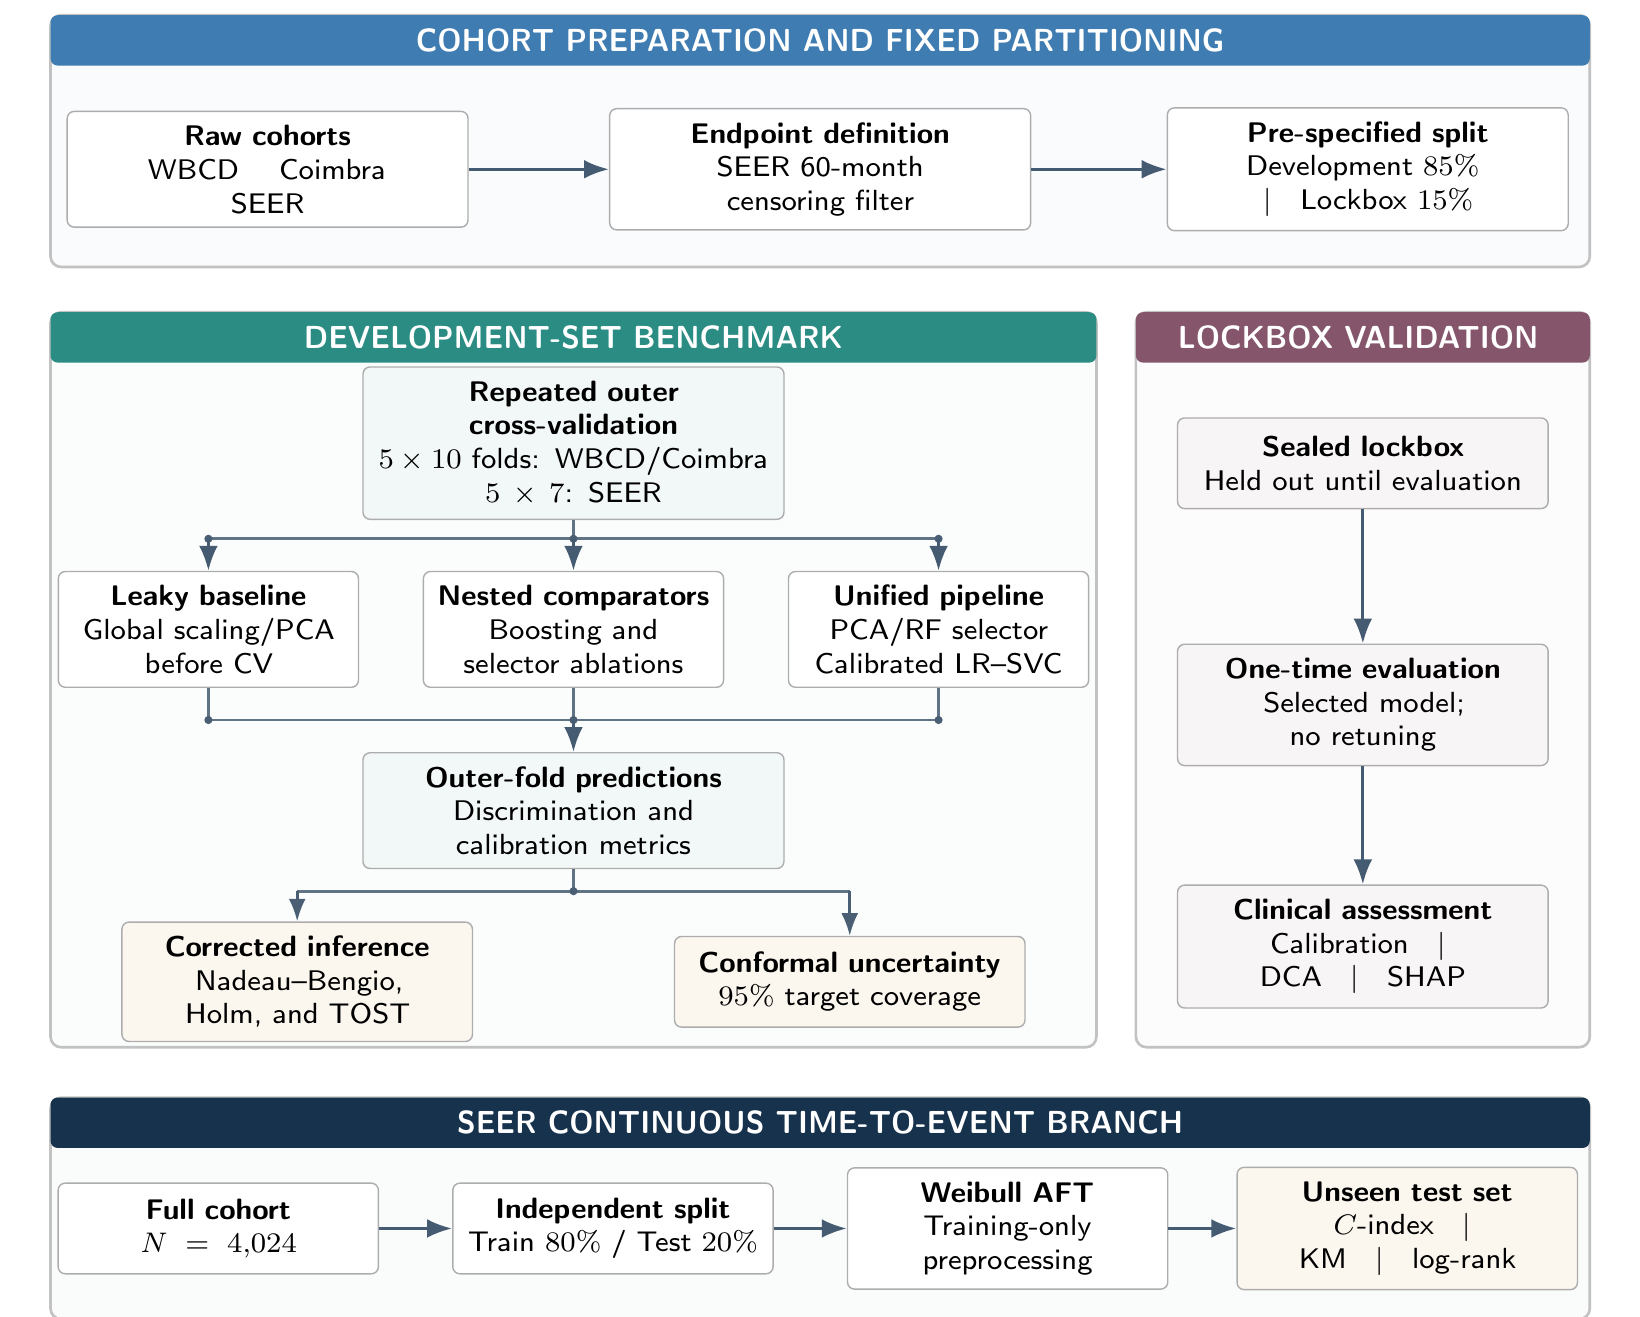
\includegraphics[width=0.9\textwidth]{figs/fig1_workflow.png}
\caption{Schematic overview of the TRUST-BC workflow. The upper lane fixes cohort endpoints (for SEER, the fixed-horizon 60-month label with exclusion of patients censored before 60 months) and partitions before any model development. The central lanes separate repeated nested benchmarking (including the architecture-matched Nested PCA-only comparator) from the sealed lockbox, which is opened once after model selection. The lower lane is the independent SEER time-to-event analysis on the full survival cohort.}\label{fig:workflow}
\end{figure}

\subsection{Baseline Architectures and Leakage Simulation}\label{sec:baseline-architectures-and-lea}
We benchmarked the Unified pipeline against tuned XGBoost and LightGBM and against nested PCA-only and RF-only ablations. A \emph{leaky baseline} performs global feature scaling and PCA on the entire development set before cross-validation, mimicking a common preprocessing error, and fits the same LR--SVC ensemble with $C=1$. Because the Unified pipeline can also select RF features and tunes $C$, the Unified-versus-Leaky contrast combines the effect of leakage with the effect of adaptive feature selection. The \emph{architecture-matched} contrast is Nested PCA-only versus Leaky: both use PCA to the same dimension and the same ensemble, and differ only in whether scaling and PCA are fitted inside the folds (and in inner tuning of $C$). We report this contrast as a post hoc descriptive analysis of the leakage effect. Gradient boosting grids explored $n\_\text{estimators}\in\{50,100\}$, maximum depth $\in\{3,5\}$ and learning rate $\in\{0.01,0.1\}$; for SEER, scale\_pos\_weight was set per fold to the training class ratio. All searches used single-threaded execution for bit-identical reproducibility.

\subsection{Resampled Statistical Testing, Confidence Intervals, and TOST Equivalence}\label{sec:resampled-statistical-testing-}
Performance differences $d_j=s_j^{\text{A}}-s_j^{\text{B}}$ across outer folds were assessed with the Nadeau--Bengio corrected variance~\cite{nadeau2003}:
\begin{equation}
\widehat{\operatorname{Var}}_{\text{corr}}(\bar{d})=S^2\Big(\frac{1}{n}+\frac{n_{\text{test}}}{n_{\text{train}}}\Big)=S^2\Big(\frac{1}{n}+\frac{1}{K-1}\Big)
\end{equation}
with $n$ outer folds ($n=50$ or 35) and $K=5$, and $t=\bar{d}/\sqrt{\widehat{\operatorname{Var}}_{\text{corr}}}$ referred to a $t_{n-1}$ distribution. A 95\% CI for each cross-validated performance estimate was obtained from the same corrected variance, as mean $\pm\,t_{n-1,0.975}\sqrt{\widehat{\operatorname{Var}}_{\text{corr}}}$, because a naive bootstrap over fold scores treats correlated folds as independent and understates uncertainty. Lockbox CIs were obtained by a stratified bootstrap of patients ($B=2{,}000$)~\cite{efron1993}, by the Wilson method for proportions.

The pre-specified Holm--Bonferroni family~\cite{holm1979} comprised five comparisons: XGBoost vs.\ Leaky, LightGBM vs.\ Leaky, Unified vs.\ XGBoost, Unified vs.\ LightGBM, and Unified vs.\ Leaky. Nested PCA-only and RF-only are descriptive ablations outside the family. Equivalence of the Unified and leaky pipelines was assessed by TOST~\cite{schuirmann1987,walker2011} with margins chosen a priori as pragmatic tolerances ($\Delta=0.02$ accuracy; $\Delta=0.01$ AUROC), not as validated clinical non-inferiority thresholds:
\begin{equation}
t_1=\frac{\bar{d}+\Delta}{\sqrt{\widehat{\operatorname{Var}}_{\text{corr}}}},\quad t_2=\frac{\bar{d}-\Delta}{\sqrt{\widehat{\operatorname{Var}}_{\text{corr}}}},\quad p_{\text{TOST}}=\max\{F_{t_{n-1}}(-t_1),F_{t_{n-1}}(t_2)\}.
\end{equation}

\subsection{Distribution-Free Conformal Prediction}\label{sec:distribution-free-conformal-pr}
Inductive split conformal prediction was applied~\cite{angelopoulos2021,vovk2005}. Hyperparameters of the conformal model were selected once by the inner search on $\mathcal{D}_{\text{dev}}$. In each of 100 iterations, $\mathcal{D}_{\text{dev}}$ was split (stratified) into a proper training subset (60\%), a calibration subset (20\%) and a test subset (20\%); calibration subsets contained 97 patients (36 events) for WBCD, 20 (11) for Coimbra and \seerNcal{} (\seerNcalEv) for SEER. Nonconformity scores were $s_i=1-\hat{P}(Y=y_i\mid x_i)$; at $\alpha=0.05$ the cut-off $\hat{q}$ was the $\lceil(n_{\text{cal}}+1)(1-\alpha)\rceil/n_{\text{cal}}$ empirical quantile, and prediction sets were
\begin{equation}
\mathcal{C}(x_{\text{new}})=\{y\in\{0,1\}:1-\hat{P}(Y=y\mid x_{\text{new}})\le\hat{q}\}.
\end{equation}
Sets were categorised as empty ($|\mathcal{C}|=0$), singleton ($|\mathcal{C}|=1$) or ambiguous ($|\mathcal{C}|=2$). The guarantee is marginal: on average over exchangeable patients, sets contain the true label with probability at least $1-\alpha$; it does not provide per-patient or per-subgroup error bounds. For the lockbox, the selected model was refitted on 80\% of $\mathcal{D}_{\text{dev}}$ and the remaining 20\% served as the conformal calibration set.

\subsection{Probability Calibration and Decision Curve Analysis}\label{sec:probability-calibration-and-de}
Probabilities were evaluated using (i) the Brier score; (ii) ECE over $M=10$ uniform bins~\cite{vancalster2019}, $\text{ECE}=\sum_m \frac{|B_m|}{N}|\text{acc}(B_m)-\text{conf}(B_m)|$; (iii) calibration slope and intercept from $\operatorname{logit}P(Y=1\mid\hat{p})=\beta_0+\beta_1\operatorname{logit}(\hat{p})$ (ideal $\beta_1=1$, $\beta_0=0$), and calibration-in-the-large (CITL, the intercept with $\operatorname{logit}\hat{p}$ as offset; ideal 0, negative values indicate overprediction); and (iv) DCA over $p_t\in[0.01,0.99]$~\cite{vickers2006}, $\text{NB}(p_t)=\frac{TP}{N}-\frac{FP}{N}\frac{p_t}{1-p_t}$.

Design choices were informed by the four PROBAST+AI domains~\cite{moons2025probast}. Because PROBAST+AI is an appraisal tool rather than a reporting checklist, we provide an author self-assessment in Supplementary Table~S2, stratified by cohort and by development versus evaluation, and do not claim a low risk of bias.

\subsection{Fairness Assessment}\label{sec:fairness-assessment}
To assess whether performance differed across sociodemographic groups, we evaluated discrimination (AUROC), calibration (CITL and slope), sensitivity, specificity and conformal coverage in the SEER cohort by race (White, Black, Other [American Indian/Alaska Native, Asian/Pacific Islander]) and by age group ($<$50, 50--59, 60--69 years), using per-patient out-of-fold predictions averaged over the seven cross-validation repeats and stratified bootstrap CIs ($B=2{,}000$). No fairness constraints or group-specific thresholds were applied. Race and age were retained as predictors because they are established prognostic factors; subgroup analysis was used to detect differential performance. WBCD contains no sociodemographic variables, and Coimbra subgroups are too small for meaningful estimates.

\subsection{Penalised Parametric Survival Modelling and Risk Stratification}\label{sec:penalised-parametric-survival-}
To model continuous prognostic trajectories in SEER, we fitted a penalised Weibull AFT model (lifelines):
\begin{equation}
\ln T=\mu+\beta^{\top}\tilde{x}+\sigma\epsilon,
\end{equation}
with $\epsilon$ following the standard extreme-value distribution and an L2 penalty ($\lambda=0.1$). Discrimination was measured by Harrell's C-index on the independent 20\% survival test partition ($n=805$), which is separate from the 15\% classification lockbox. Because lifelines was not available for the revision analysis, the C-index CI was obtained by bootstrapping ($B=2{,}000$) the test partition using an independent re-implementation of the same model, which reproduced the reported C-index to within 0.002. Test patients were dichotomised at the median predicted survival of the training partition and survival curves compared by the log-rank test:
\begin{equation}
\chi^2=\frac{\big(\sum_j(O_{1j}-E_{1j})\big)^2}{\sum_j V_{1j}}.
\end{equation}

\subsection{Interpretability}\label{sec:interpretability}
Model attributions on the lockbox were computed with Kernel SHAP~\cite{lundberg2017} (background of 50 training patients) for WBCD and Coimbra. For the corrected SEER analysis, Shapley values for the same subsample of 100 lockbox patients and the same background were estimated by Monte Carlo permutation sampling (40 permutations per patient)~\cite{strumbelj2014}, which targets the same interventional Shapley values as Kernel SHAP.

\section{Results}\label{sec:results}
\subsection{Participants}\label{sec:participants}
Participant flow is shown in Supplementary Figure~S1. WBCD and Coimbra had no exclusions. Of the 4,024 SEER patients, 754 were alive with fewer than 60 months of follow-up and were excluded from the classification cohort, leaving 3,270 patients (458 deaths within 60 months; 158 later deaths counted as 5-year survivors), of whom 2,779 (389 events) formed the development set and 491 (69 events) the lockbox. All 4,024 patients entered the survival branch (3,219 training, 805 test with 123 deaths). Development and lockbox partitions were well balanced (absolute standardised mean differences $\le$0.12 for WBCD and \seerMaxSMD{} for SEER; up to 0.38 for Coimbra, reflecting the very small lockbox of 18 patients; Supplementary Table~S3). In the SEER classification cohort, 60-month mortality was 23.9\% among Black, 13.7\% among White and 8.2\% among Other-race patients, and Black patients more often had N3 disease (17.3\% vs 12.5\%) and estrogen-receptor-negative tumours (12.8\% vs 6.9\%) than White patients (Supplementary Table~S3b).

\subsection{Multicohort Benchmark and Equivalence Results}\label{sec:multicohort-benchmark-and-equi}
Cross-validated performance is detailed in Table~\ref{tab:bench} and Figure~\ref{fig:main}. The Unified pipeline reached 97.08\% accuracy on WBCD, 71.35\% on Coimbra, and an AUROC of \seerUniAUC{} on SEER.

\begin{table}[!htbp]
\centering\footnotesize
\caption{Cross-validated multicohort benchmark (primary metric: accuracy for WBCD and Coimbra, AUROC for SEER).}\label{tab:bench}
\setlength{\tabcolsep}{3pt}
\begin{tabular}{@{}llllllll@{}}
\toprule
\textbf{Cohort} & \textbf{Pipeline} & \textbf{Mean $\pm$ SD} & \textbf{95\% CI\textsuperscript{a}} & \textbf{\makecell{Holm $p$\\vs Leaky}} & \textbf{\makecell{Holm $p$\\vs Unified}} & \textbf{$p_{\text{TOST}}$\textsuperscript{b}} & \textbf{Brier / ECE}\\
\midrule
WBCD & Leaky baseline & 96.85\% $\pm$ 1.65 & 95.13--98.57 & -- & -- & -- & 0.024 / 0.020\\
($n=569$) & Tuned XGBoost & 95.20\% $\pm$ 2.08 & 93.03--97.37 & 0.4448 & 0.3292 & -- & 0.034 / 0.012\\
& Tuned LightGBM & 95.82\% $\pm$ 2.30 & 93.41--98.22 & 0.6642 & 0.6615 & -- & 0.033 / 0.016\\
& Nested PCA-only & 97.16\% $\pm$ 1.65 & 95.44--98.88 & -- & -- & -- & 0.023 / 0.018\\
& Nested RF-only & 95.94\% $\pm$ 1.94 & 93.92--97.97 & -- & -- & -- & 0.031 / 0.016\\
& Unified & 97.08\% $\pm$ 1.67 & 95.34--98.82 & 0.6642 & -- & 0.0002$^{*}$ & 0.024 / 0.017\\
\midrule
Coimbra & Leaky baseline & 62.73\% $\pm$ 10.70 & 51.56--73.91 & -- & -- & -- & 0.208 / 0.087\\
($n=116$) & Tuned XGBoost & 75.64\% $\pm$ 9.72 & 65.49--85.79 & 0.2494 & 0.9897 & -- & 0.174 / 0.062\\
& Tuned LightGBM & 74.78\% $\pm$ 10.66 & 63.65--85.92 & 0.2371 & 0.9897 & -- & 0.178 / 0.071\\
& Nested PCA-only & 63.25\% $\pm$ 10.88 & 51.89--74.61 & -- & -- & -- & 0.212 / 0.062\\
& Nested RF-only & 72.37\% $\pm$ 8.20 & 63.81--80.93 & -- & -- & -- & 0.183 / 0.062\\
& Unified & 71.35\% $\pm$ 8.70 & 62.27--80.43 & 0.2657 & -- & 0.9059 & 0.186 / 0.054\\
\midrule
SEER & Leaky baseline & \seerLeakAUC{} $\pm$ \seerLeakSD & \seerLeakCI & -- & -- & -- & \seerLeakBE\\
5-year & Nested PCA-only & \seerPCAAUC{} $\pm$ \seerPCASD & \seerPCACI & -- & -- & -- & \seerPCABE\\
($N=3{,}270$) & Nested RF-only & \seerRFAUC{} $\pm$ \seerRFSD & \seerRFCI & -- & -- & -- & \seerRFBE\\
& Unified & \seerUniAUC{} $\pm$ \seerUniSD & \seerUniCIs & \seerUniP$^{\dagger}$ & -- & \seerUniTOST & \seerUniBE\\
\bottomrule
\end{tabular}
\par\vspace{3pt}{\footnotesize\raggedright\setlength{\parskip}{1pt}
\par Values after $\pm$ are standard deviations across outer folds (50 for WBCD/Coimbra, 35 for SEER).
\par\textsuperscript{a}Nadeau--Bengio corrected 95\% intervals~\cite{nadeau2003}.
\par\textsuperscript{b}TOST only for the pre-specified Unified versus Leaky comparison ($\Delta=0.02$ accuracy; $\Delta=0.01$ AUROC). $^{*}$Equivalence established at $\alpha=0.05$ (TOST is not part of the Holm-adjusted superiority family).
\par $^{\dagger}$SEER (corrected 5-year label): gradient boosting baselines were not re-run for the corrected endpoint, so the Holm family reduces to the single Unified versus Leaky comparison (unadjusted corrected $t$-test). Results for all six pipelines under the v1.0 label are in Supplementary Table~S8.
\par Pooled out-of-fold AUROCs for WBCD (0.993) and Coimbra (0.793) are descriptive secondary estimates.
\par}
\end{table}

\begin{figure}[p]
\centering
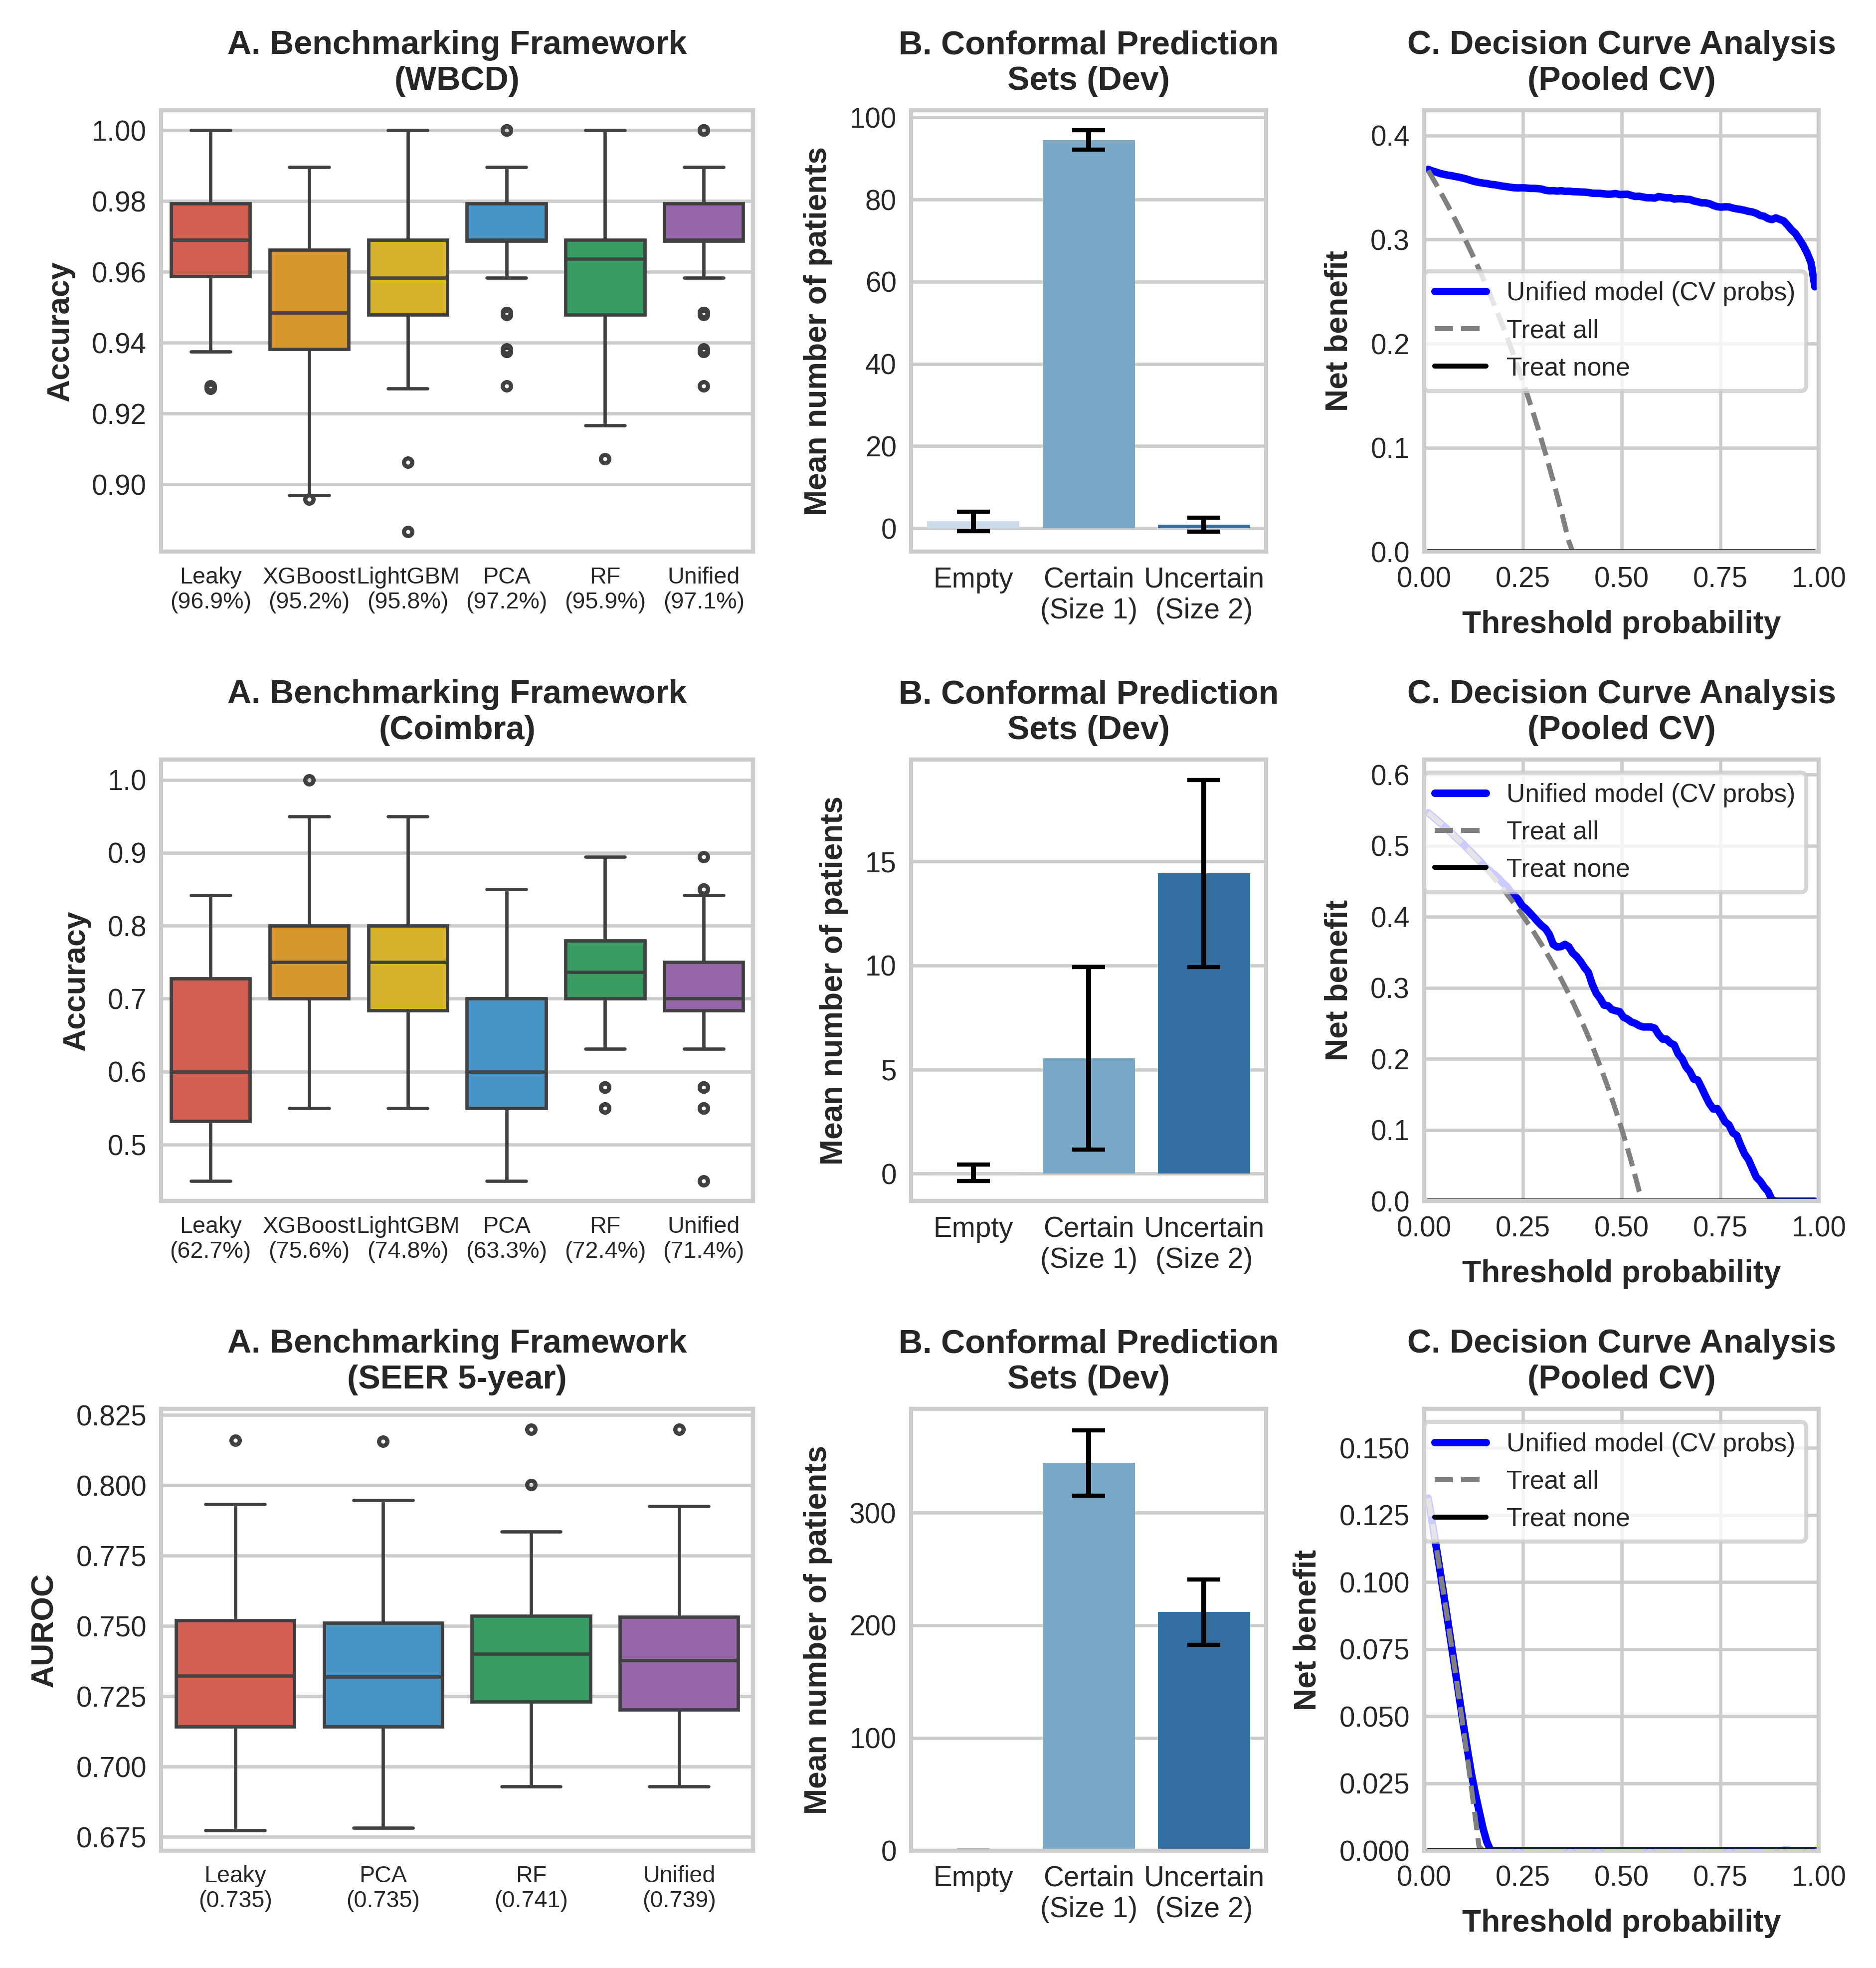
\includegraphics[width=\textwidth]{figs/fig2_benchmark.png}
\caption{Cross-validated benchmark performance distributions across outer folds (A), conformal prediction-set cardinality at 95\% target coverage, shown as the mean number of development-set test patients over 100 calibration iterations with SD error bars (B), and decision curve analysis on pooled out-of-fold predictions (C). Rows: WBCD, Coimbra, and SEER 5-year (corrected fixed-horizon label; gradient boosting baselines not re-run).}\label{fig:main}
\end{figure}

On \textbf{WBCD}, the Unified pipeline was formally equivalent to the leaky baseline ($p_{\text{TOST}}=0.0002$; difference $+0.23$ percentage points, 90\% CI $-0.55$ to $+1.01$). On \textbf{Coimbra}, Unified accuracy (71.35\%) exceeded the leaky baseline (62.73\%) and Nested PCA (63.25\%) and was comparable to the tree ensembles (72.37--75.64\%); TOST did not establish equivalence ($p_{\text{TOST}}=0.9059$), because the Unified pipeline was \emph{better} than the leaky baseline (difference $+8.62$ points, 90\% CI $+0.30$ to $+16.94$). On \textbf{SEER}, the Unified AUROC was \seerUniAUC{} (\seerUniCI), similar to Nested RF (\seerRFAUC); TOST did not establish equivalence within $\pm0.01$ ($p_{\text{TOST}}=\seerUniTOST$; difference \seerDiffUL, 90\% CI \seerDiffULci).

\paragraph{Architecture-matched leakage contrast.} Table~\ref{tab:leak} separates the leakage effect from the selector effect. When the architecture was held fixed (Nested PCA-only versus Leaky), fitting scaling and PCA inside the folds changed performance by $+0.31$ points in WBCD, $+0.52$ points in Coimbra and \seerDiffPL{} AUROC in SEER, with all 95\% CIs including zero; in SEER the two pipelines were formally equivalent within $\pm0.01$ AUROC ($p_{\text{TOST}}<0.001$). Global scaling/PCA leakage therefore produced no measurable optimism in these cohorts, and the non-equivalence of the Unified pipeline in Coimbra and SEER reflects the gain from adaptive RF feature selection, not leakage.

\begin{table}[!htbp]
\centering\small
\caption{Leakage and selector contrasts in the cohort-specific primary metric (Nadeau--Bengio corrected intervals).}\label{tab:leak}
\begin{tabularx}{\textwidth}{@{}P{3.3cm}YYP{1.5cm}@{}}
\toprule
\textbf{Cohort (metric)} & \textbf{Nested PCA $-$ Leaky: leakage only (95\% CI)} & \textbf{Unified $-$ Leaky: leakage + selector (90\% CI)} & \textbf{$p_{\text{TOST}}$ (Unified vs Leaky)}\\
\midrule
WBCD (accuracy, points) & $+$0.31 ($-$0.54 to $+$1.16) & $+$0.23 ($-$0.55 to $+$1.01) & 0.0002\\
Coimbra (accuracy, points) & $+$0.52 ($-$4.68 to $+$5.72) & $+$8.62 ($+$0.30 to $+$16.94) & 0.9059\\
SEER 5-year (AUROC) & \seerDiffPL{} (\seerDiffPLci) & \seerDiffUL{} (\seerDiffULci) & \seerUniTOST\\
\bottomrule
\end{tabularx}
\end{table}

\paragraph{Calibration.} Pooled ECE for SEER (\seerUniECE) was similar to that of the leaky baseline (\seerLeakECE) and higher than for WBCD (0.017) and Coimbra (0.054). SEER probabilities were systematically too high: mean predicted risk was \seerMeanPred\% against an observed 60-month mortality of 14.0\% (calibration-in-the-large \seerCITL; slope \seerSlope). This overprediction is the expected consequence of balanced class weighting in a cohort with 14\% prevalence and shows that leakage removal does not by itself produce calibrated probabilities; both diagnostics should be reported jointly.

\paragraph{Decision curves.} For WBCD and Coimbra, the Unified pipeline provided higher net benefit than both default strategies across $p_t\in[0.10,0.40]$ (Figure~\ref{fig:main}). For SEER, net benefit exceeded both defaults only between $p_t\approx\seerDCAlo$ and \seerDCAhi{} and was zero or negative above approximately 0.17 (Figure~\ref{fig:main}c), so the claim of clinical utility across $p_t\in[0.10,0.40]$ made for the diagnostic cohorts does not hold for the registry model; this is consistent with its overprediction and moderate discrimination.

\paragraph{Architecture selection.} PCA was selected in 47/50 WBCD folds (94\%), consistent with high collinearity among continuous morphological features. RF was selected in 46/50 Coimbra folds (92\%) and in \seerRFfolds/35 SEER folds; the five-seed winner's-curse check selected RF in all five SEER seeds.

\subsection{Conformal Prediction and Lockbox Validation}\label{sec:conformal-prediction-and-lockb}
Clinical diagnostic panels (pooled ROC, precision--recall, reliability diagrams and feature-selection stability) are shown in Figure~\ref{fig:clin}. Empirical conformal coverage was 96.53\% for WBCD, 95.70\% for Coimbra and \seerConfCov\% for SEER, consistent with the nominal 95\%. Singleton sets comprised 97.40\% of WBCD, 27.70\% of Coimbra and \seerConfSingle\% of SEER predictions, and ambiguous sets 0.90\%, 72.10\% and \seerConfAmb\%, respectively. Empty sets were rare for WBCD (1.70\%) and Coimbra (0.20\%) and absent for SEER. In SEER, coverage was markedly unequal by outcome class: 99.4\% of patients who survived 5 years but only 69.9\% of those who died were covered, so the marginal 95\% guarantee concealed substantial under-coverage of the clinically most important class. Lockbox results are shown in Table~\ref{tab:lock}.

\begin{figure}[p]
\centering
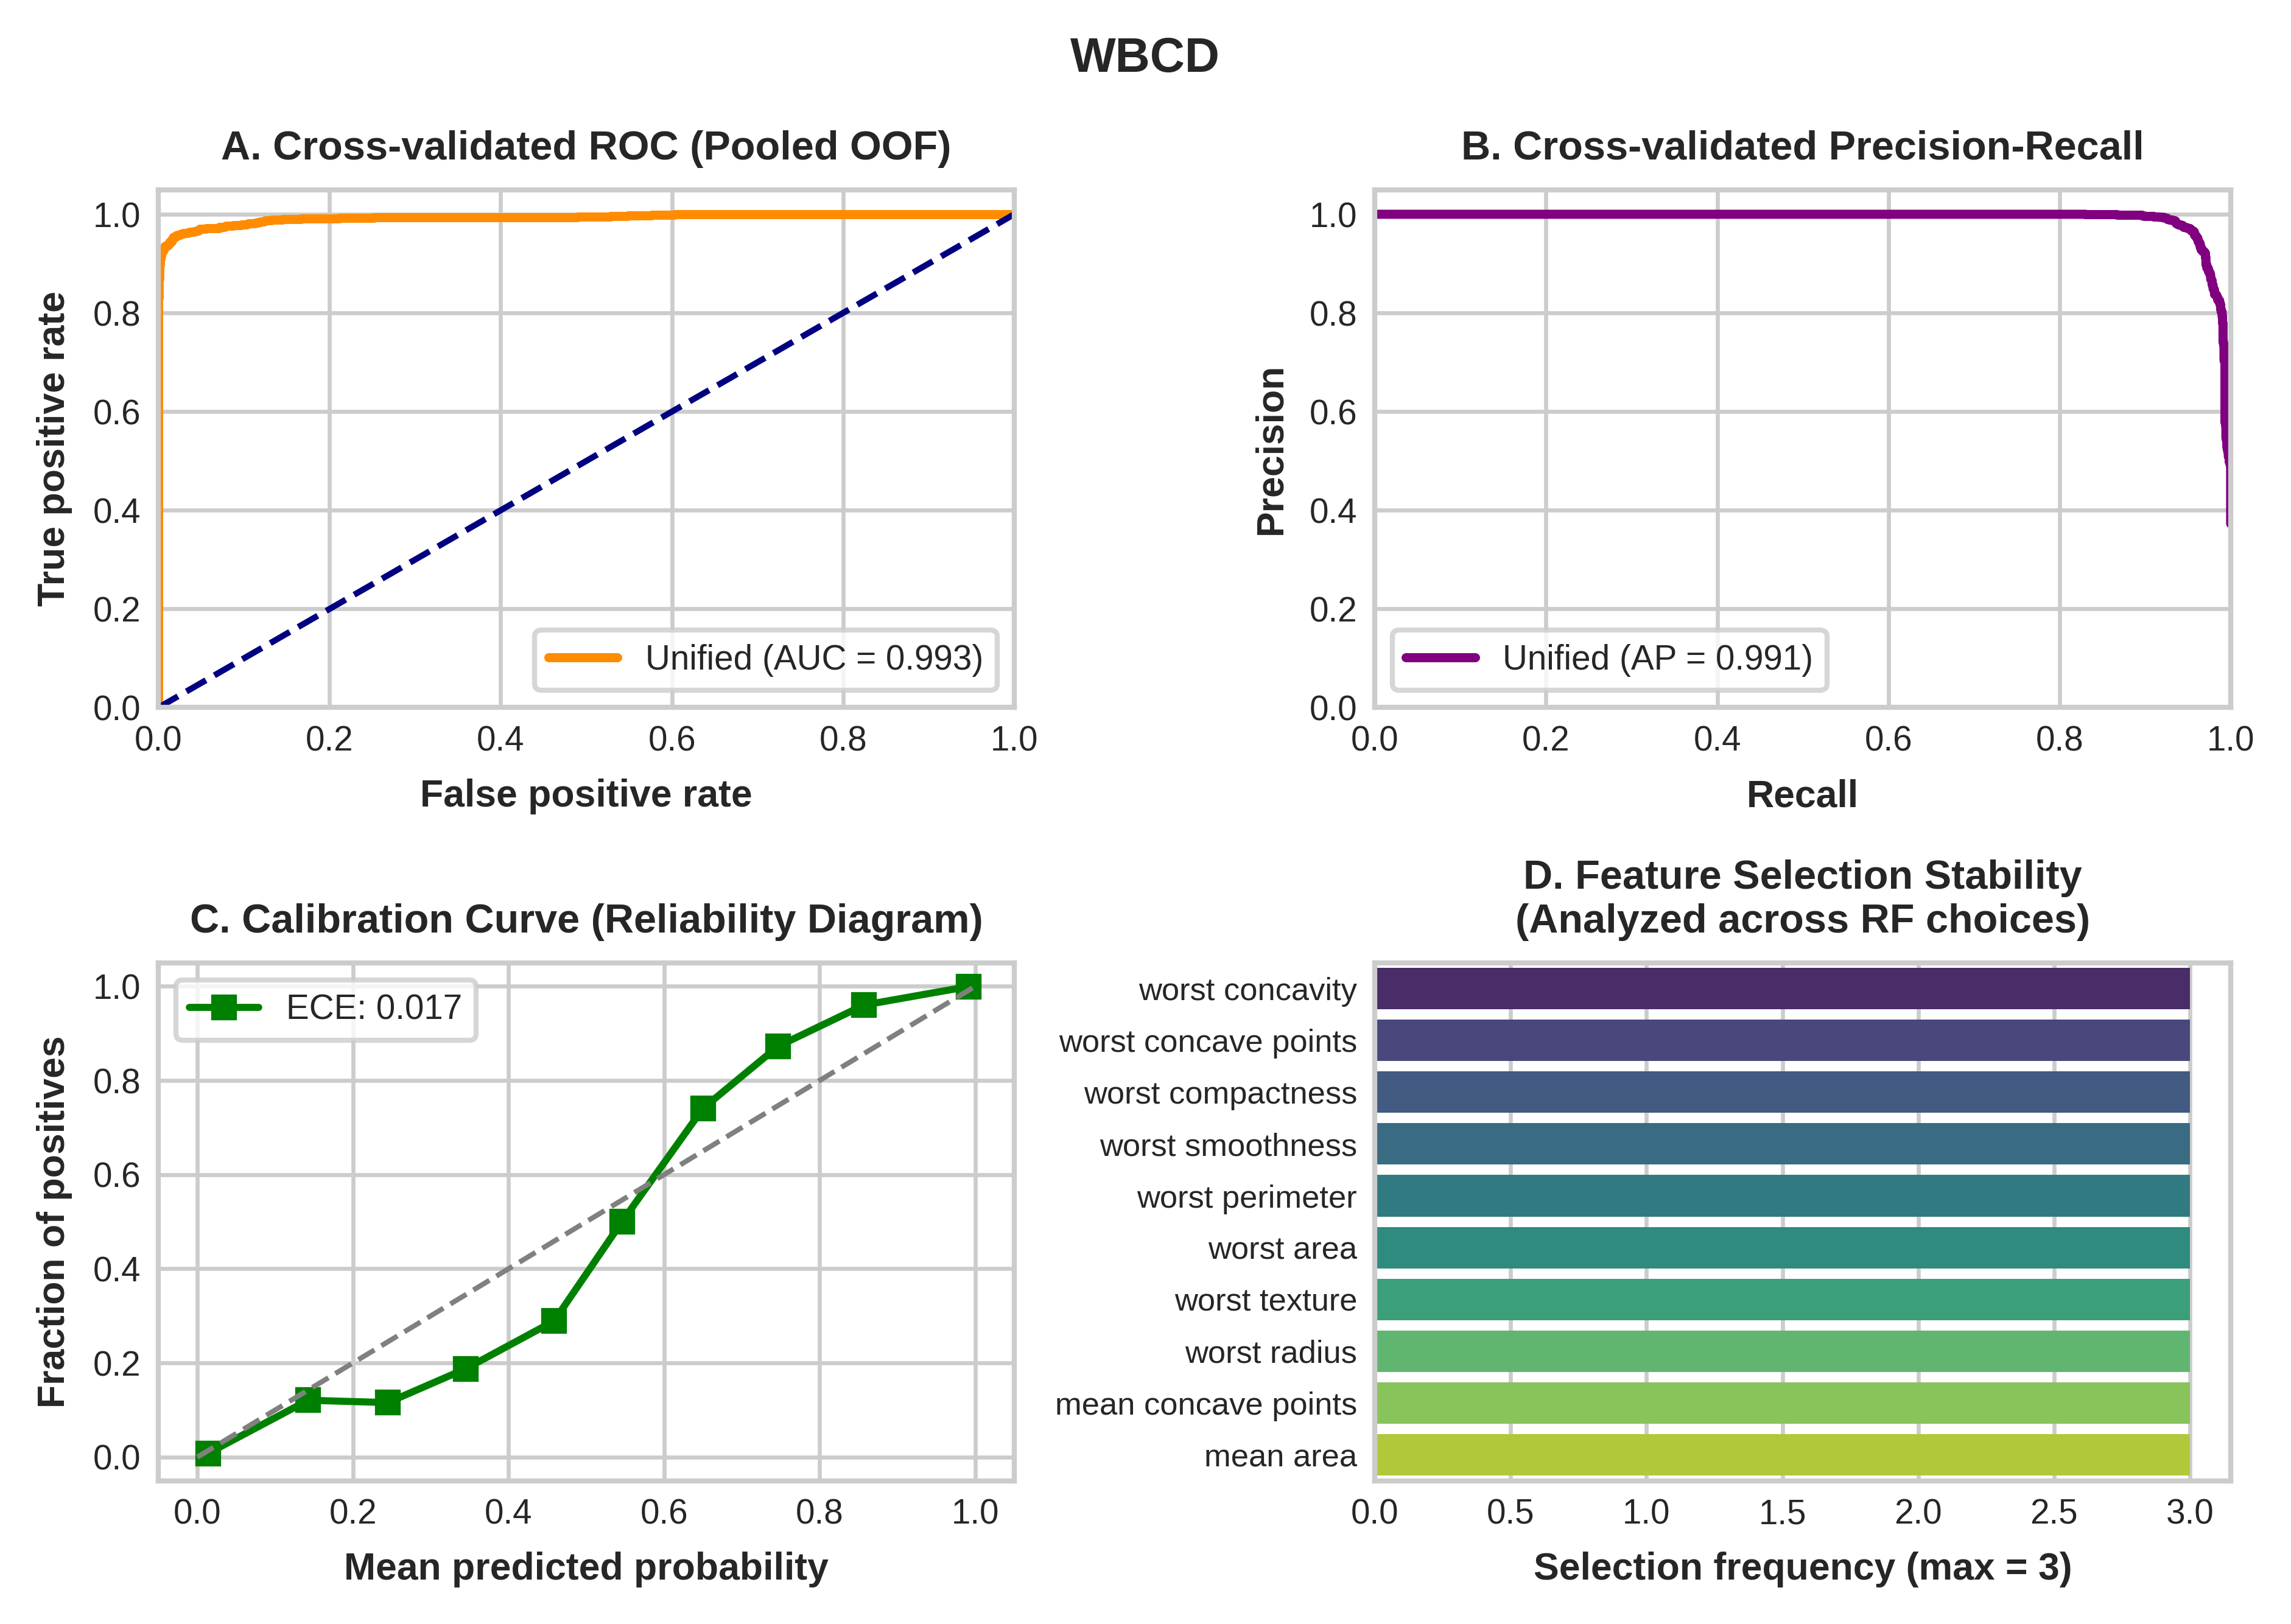
\includegraphics[width=0.96\textwidth]{figs/fig3a_clinical_wbcd.png}\\[2pt]
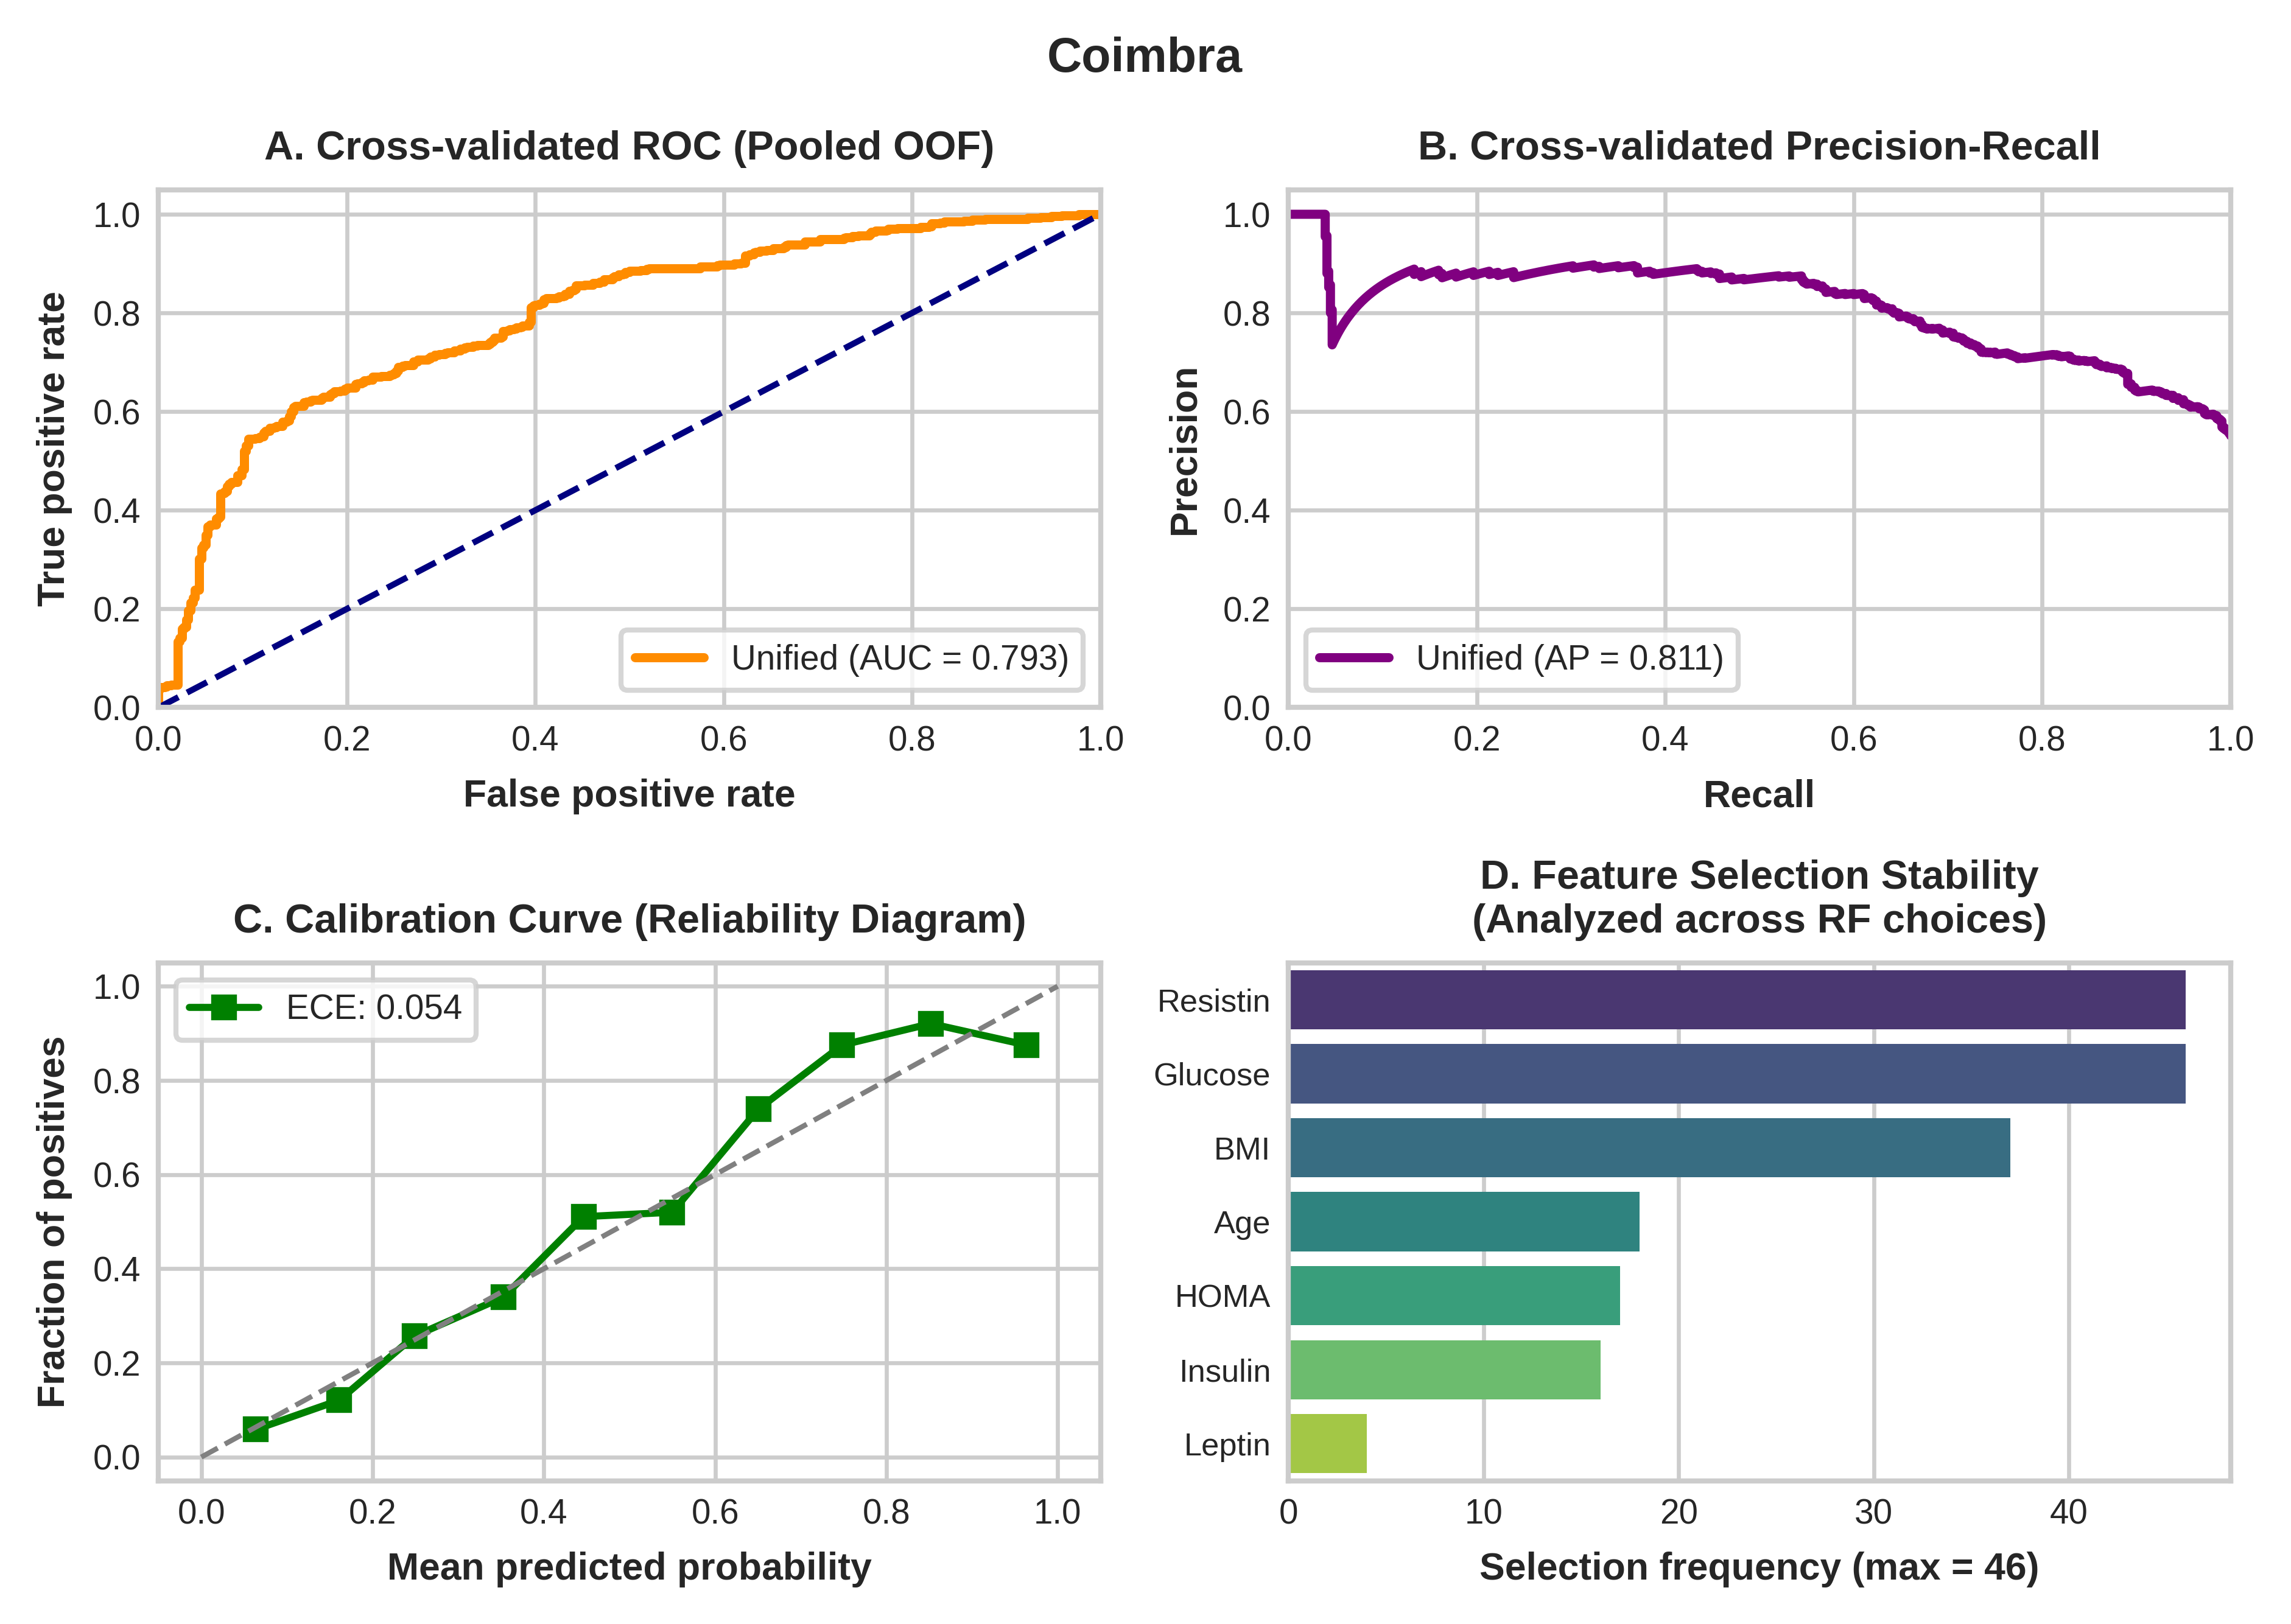
\includegraphics[width=0.96\textwidth]{figs/fig3b_clinical_coimbra.png}
\caption{Clinical diagnostic panels by cohort: (A) pooled out-of-fold ROC curve, (B) precision--recall curve, (C) reliability diagram with ECE, and (D) random-forest feature-selection frequency across the outer folds in which RF was selected. (a) WBCD; (b) Coimbra; (c) SEER 5-year on the next page. Pooled AUROCs for WBCD and Coimbra are descriptive secondary estimates.}\label{fig:clin}
\end{figure}
\begin{figure}[t!]
\ContinuedFloat
\centering
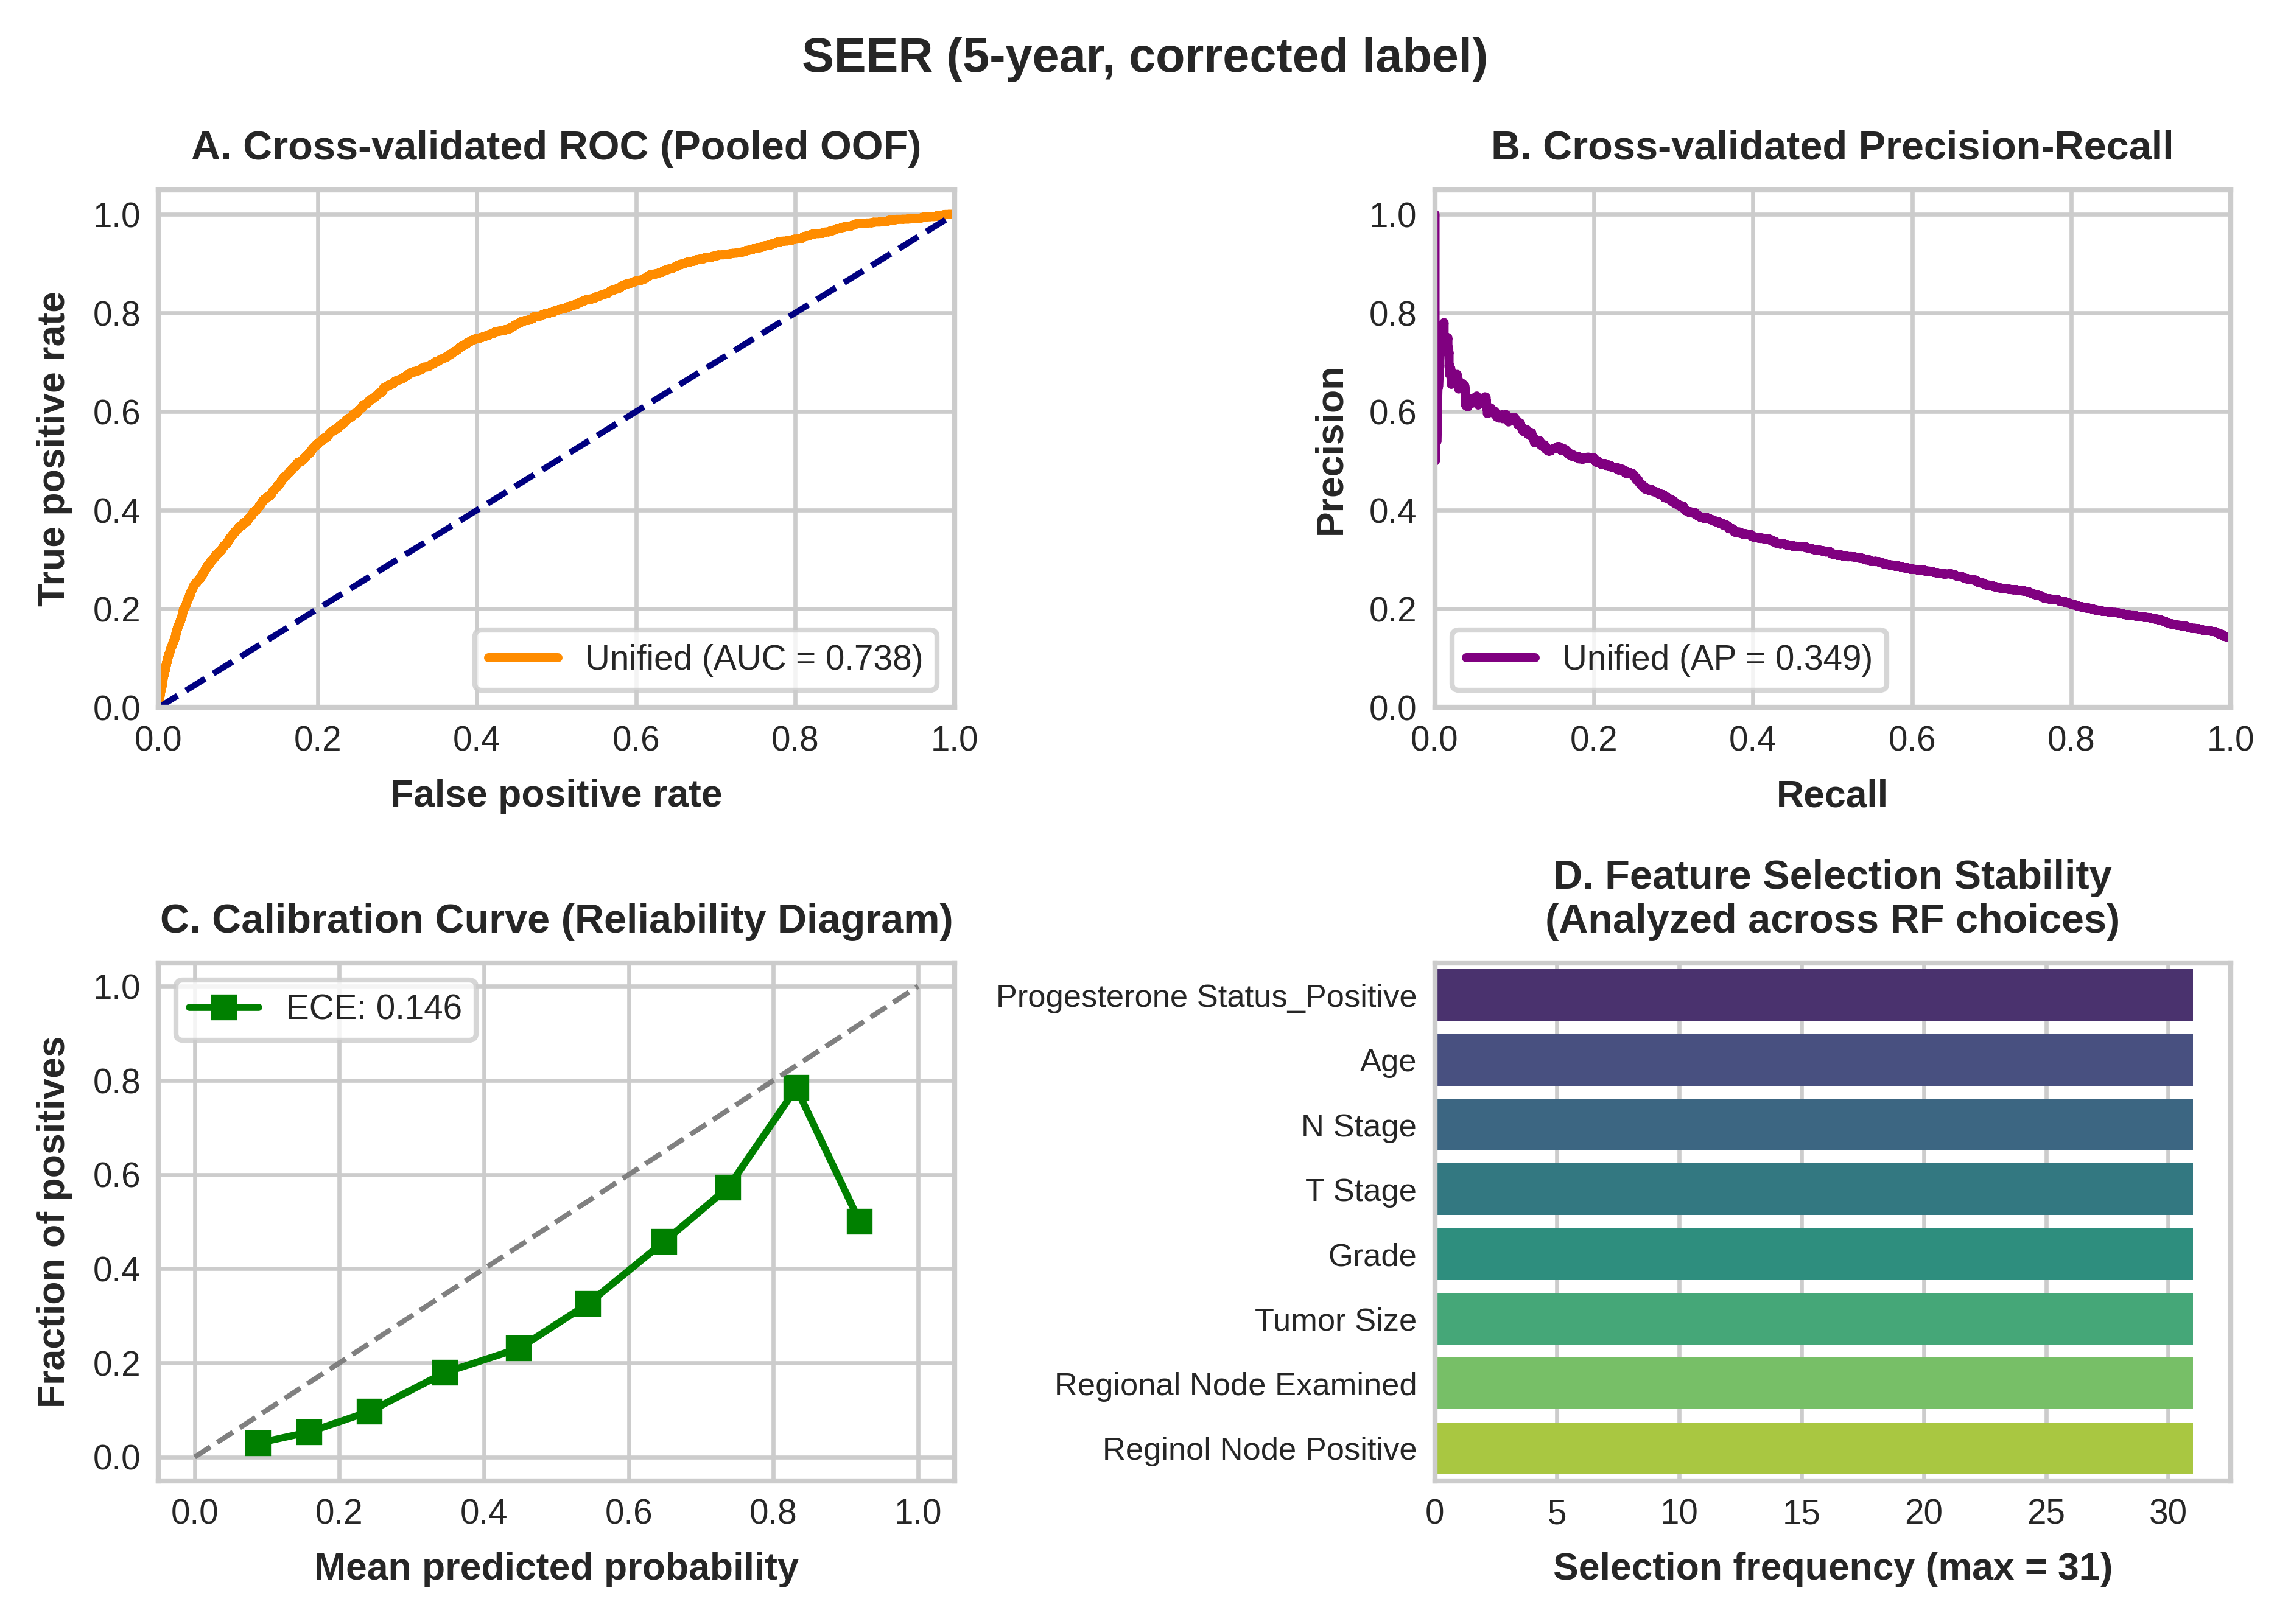
\includegraphics[width=\textwidth]{figs/fig3c_clinical_seer.png}
\caption{(continued) (c) SEER 5-year classification cohort (corrected label).}
\end{figure}

\begin{table}[!htbp]
\centering\small
\caption{Performance on the held-out lockbox partitions (15\%), with 95\% CIs.}\label{tab:lock}
\setlength{\tabcolsep}{4pt}
\begin{tabularx}{\textwidth}{@{}P{3.4cm}YYY@{}}
\toprule
\textbf{Metric} & \textbf{WBCD ($n=86$; 32 events)} & \textbf{Coimbra ($n=18$; 10 events)} & \textbf{SEER 5-year ($n=491$; 69 events)}\\
\midrule
Accuracy\textsuperscript{a} & 100.00\% (95.72--100.00) & 61.11\% (38.62--79.69) & \seerLbAcc\% (\seerLbAccCI)\\
Balanced accuracy & 100.00\% & 62.50\% & \seerLbBal\%\\
Sensitivity & 100.00\% (32/32) & 50.00\% (5/10) & \seerLbSens\\
Specificity & 100.00\% (54/54) & 75.00\% (6/8) & \seerLbSpec\\
AUROC & 1.000 (1.000--1.000)\textsuperscript{b} & 0.725 (0.450--0.975)\textsuperscript{b} & \seerLbAUC{} (\seerLbAUCCI)\textsuperscript{b}\\
Brier score & \wbcdLbBrier{} (\wbcdLbBrierCI)\textsuperscript{b} & 0.234 (0.146--0.334)\textsuperscript{b} & \seerLbBrier{} (\seerLbBrierCI)\textsuperscript{b}\\
Calibration slope ($\beta_1$) & 14.820\textsuperscript{e} & 0.632 ($-$0.29 to 9.06)\textsuperscript{c} & \seerLbSlope{} (\seerLbSlopeCI)\\
Calibration intercept ($\beta_0$) & 1.784\textsuperscript{e} & 0.257 ($-$0.14 to 5.58)\textsuperscript{c} & \seerLbInt{} (\seerLbIntCI)\\
Calibration-in-the-large & -- & -- & \seerLbCITL{} (\seerLbCITLCI)\\
Conformal coverage\textsuperscript{a} & 98.84\% (93.70--99.79) & 83.33\% (60.78--94.16) & \seerLbCov\% (\seerLbCovCI)\\
\bottomrule
\end{tabularx}
\par\vspace{3pt}{\footnotesize\raggedright\setlength{\parskip}{1pt}
\par\textsuperscript{a}Wilson intervals. \par\textsuperscript{b}Stratified bootstrap of patients ($B=2{,}000$); WBCD and Coimbra values from re-created lockbox predictions, which reproduced the reported accuracy, AUROC, Brier score and calibration coefficients exactly.
\par\textsuperscript{c}Stratified bootstrap; with 18 patients (10 events) the recalibration model is unstable and these intervals are extremely wide.
\par\textsuperscript{e}Quasi-complete separation; not interpretable as a calibration diagnostic (see text).
\par}
\end{table}

The Coimbra lockbox coverage was 83.33\% (15/18; 95\% CI 60.78--94.16), below the nominal 95\% and the development-set estimate of 95.70\%; with 18 patients this estimate has substantial uncertainty and should not by itself be interpreted as systematic under-coverage. On the WBCD lockbox, the Unified model achieved perfect discrimination; the extreme calibration slope ($\beta_1=14.82$) reflects quasi-complete separation in maximum-likelihood logistic recalibration~\cite{albert1984,heinze2002}, in which coefficients diverge with large standard errors, rather than miscalibration. We report it descriptively; Firth's penalised likelihood~\cite{heinze2002} would be an appropriate remedy. This ceiling performance is in line with previous reports on this benchmark (Street et al.~\cite{street1993} $\approx$97.0\%; Asri et al.~\cite{asri2016} $\approx$97.13\%) and with our cross-validated 97.08\%, and is not evidence of residual leakage (sample-hash overlap 0.00\%). On the SEER lockbox, AUROC was \seerLbAUC{} (\seerLbAUCCI) and sensitivity was low (\seerLbSens) at the 0.5 threshold, and the calibration intercept confirmed overprediction; the calibration slope (\seerLbSlope) was close to 1.

\subsection{Global Model Interpretability}\label{sec:global-model-interpretability}
Attributions on the lockboxes are shown in Figure~\ref{fig:shap}. Nuclear concavity, texture and perimeter features were most influential for cytopathological diagnosis (WBCD), glucose, BMI and resistin for serum metabolic classification (Coimbra), and \seerShapTop{} for 5-year mortality (SEER).

\begin{figure}[p]
\centering
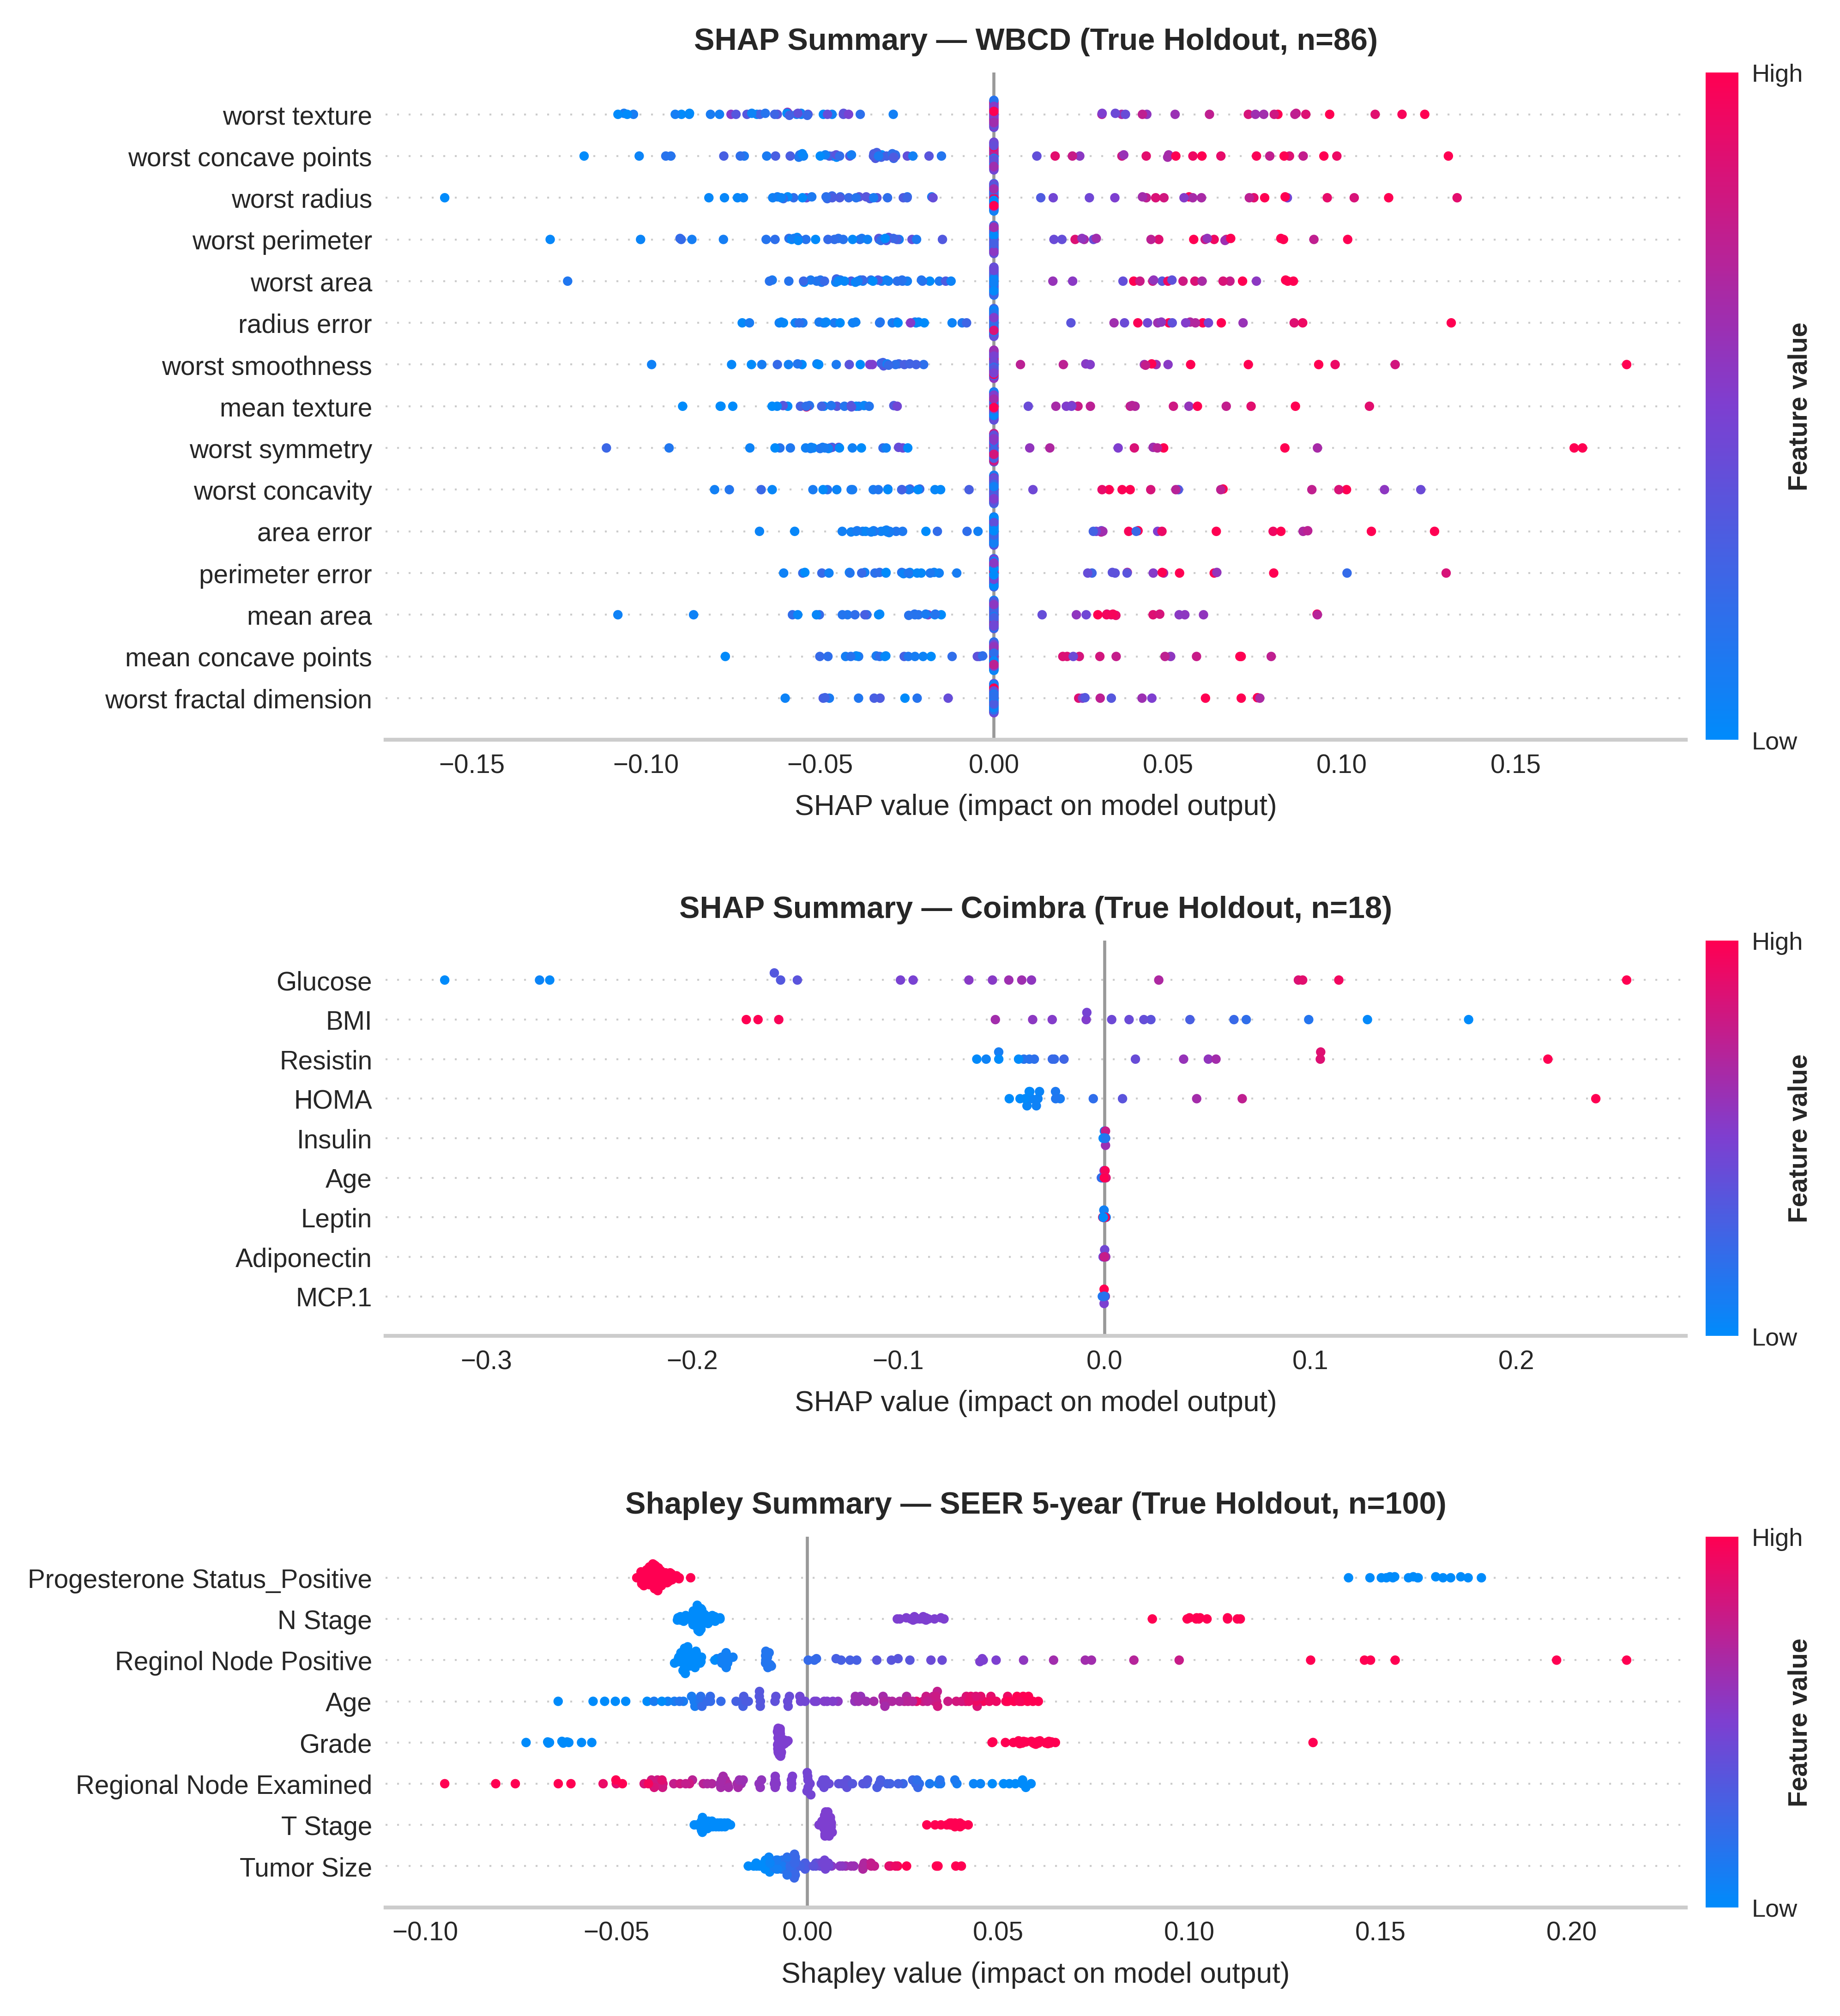
\includegraphics[width=\textwidth]{figs/fig4_shapley.png}
\caption{Shapley attributions on the held-out lockboxes, showing each feature's direction and magnitude of impact on the predicted probability (colour: feature value). WBCD and Coimbra: Kernel SHAP values from the v1.0 run; SEER 5-year: permutation Shapley values for 100 of the 491 lockbox patients. Only features with non-zero attribution are shown; for SEER these are the eight random-forest-selected features.}\label{fig:shap}
\end{figure}

\subsection{Sample-Size and Dimensionality Sensitivity}\label{sec:sample-size-and-dimensionality}
Bootstrapped learning curves over subsample fractions $\eta\in\{0.30,0.50,0.70,0.85,1.00\}$ ($B=200$) showed increasing accuracy with shrinking uncertainty for WBCD and Coimbra (Figure~\ref{fig:ss}); in Coimbra, variance remained large at full scale ($n=98$). For SEER, accuracy plateaued at 83.7--84.2\% from 30\% of the development data onward, close to the 86\% accuracy of always predicting survival, which reflects the low prevalence and the 0.5 threshold rather than a lack of data. Across component counts $d\in\{\lfloor d_0/2\rfloor,d_0,\lfloor1.5d_0\rfloor,\min(D,2d_0)\}$, performance was relatively stable in WBCD (maximum fluctuation 0.0186 accuracy). In SEER, AUROC increased with the number of retained features (from 0.696--0.722 at $d=4$ to 0.749 at $d=16$), indicating that the pre-specified heuristic ($d=8$) discarded some prognostic information. In Coimbra the selector choice mattered at low dimension ($d=2$: RF 76.50\% vs PCA 62.20\%, a 14.30-point gap) (Figure~\ref{fig:dim}), supporting automated selector optimisation for small samples.

\begin{figure}[p]
\centering
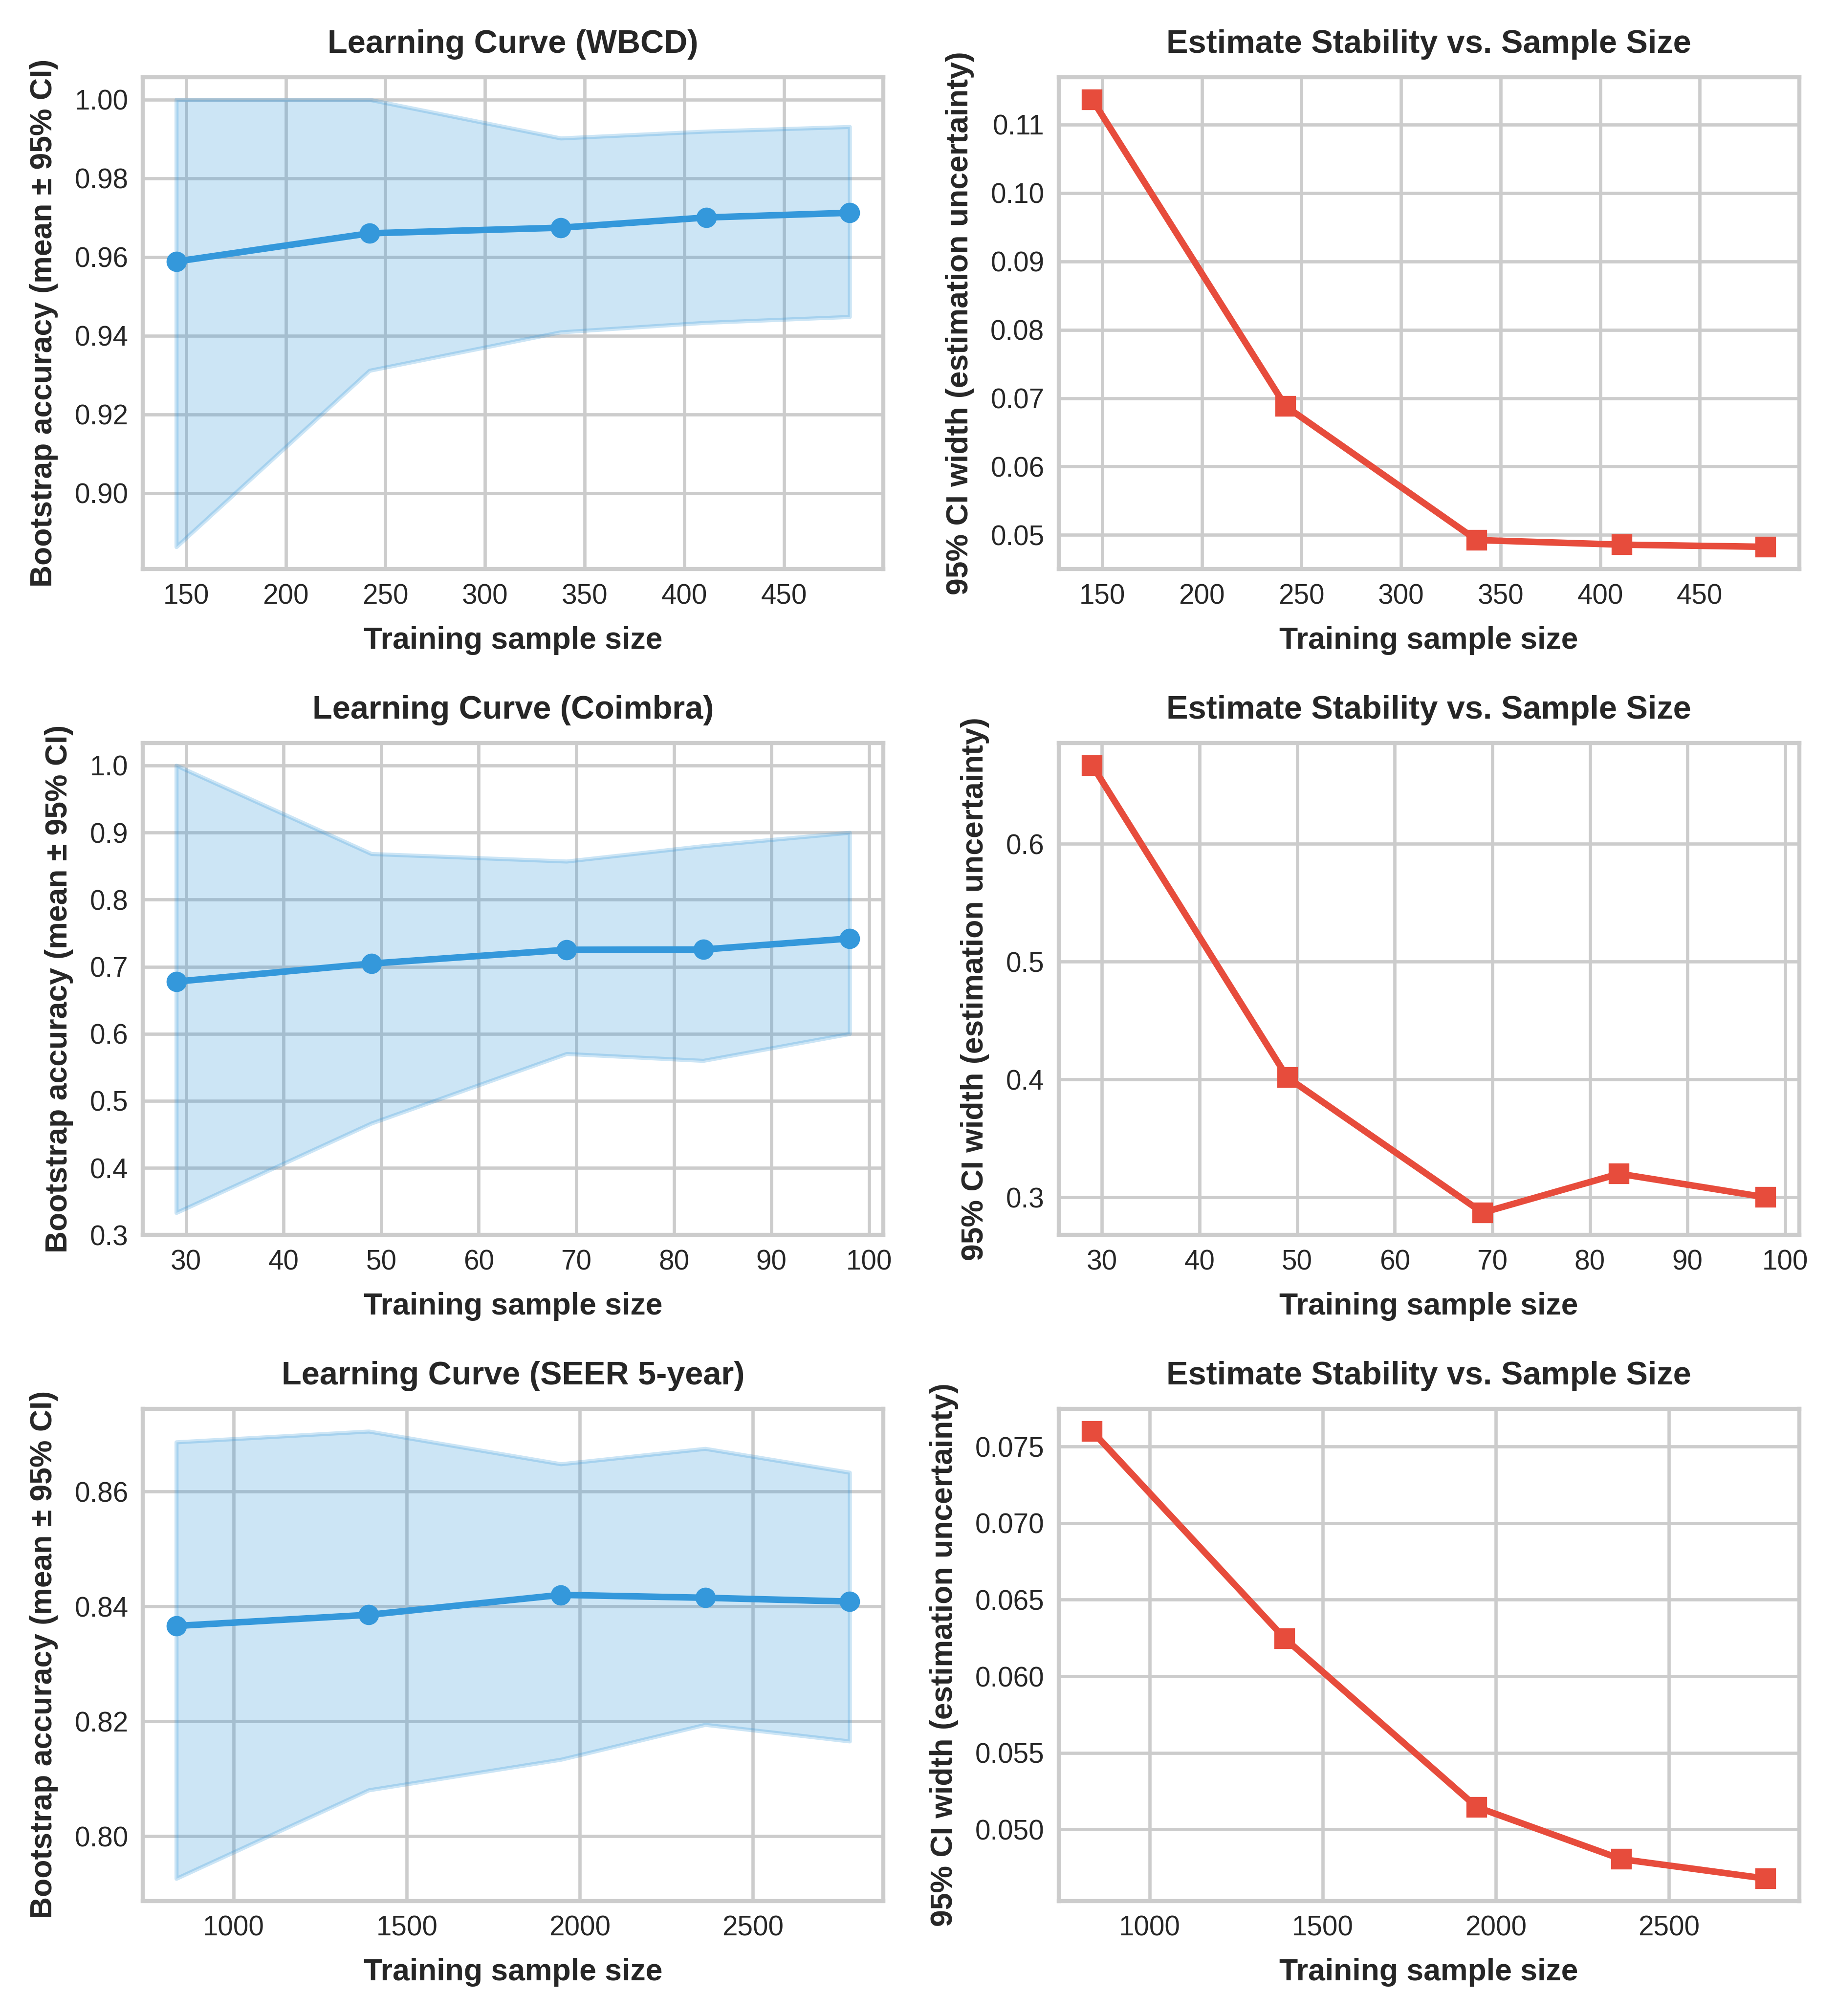
\includegraphics[width=\textwidth]{figs/fig5_sample_size.png}
\caption{Sample-size sensitivity: bootstrapped learning curves (left) and width of the 95\% bootstrap interval (right) across subsample fractions of 30\%, 50\%, 70\%, 85\% and 100\% of the development set ($B=200$). Accuracy is used in all panels for uniformity; AUROC remains the primary SEER metric elsewhere.}\label{fig:ss}
\end{figure}

\begin{figure}[htbp]
\centering
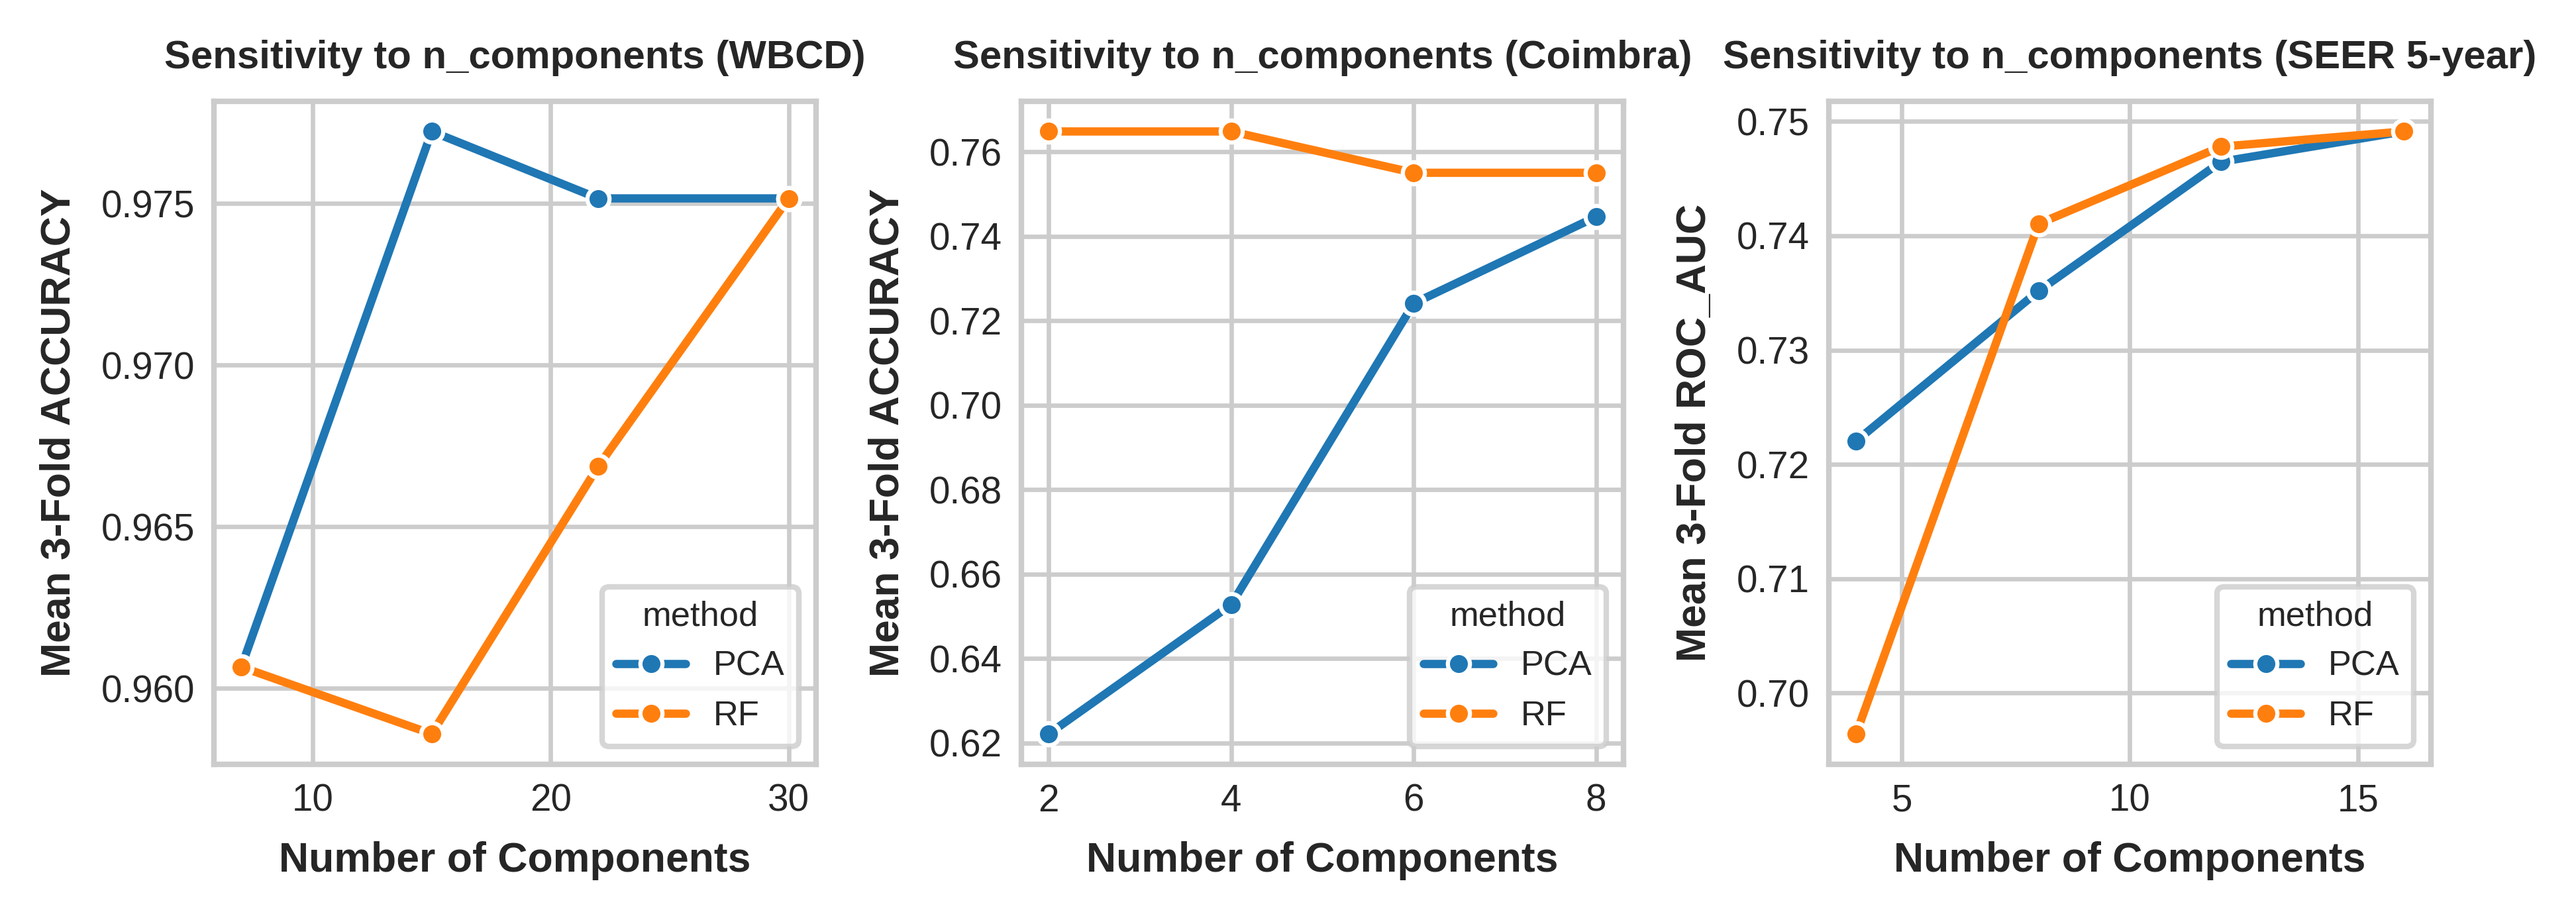
\includegraphics[width=\textwidth]{figs/fig6_dimensionality.png}
\caption{Dimensionality sensitivity: mean 3-fold performance by number of retained PCA components or random-forest-selected features.}\label{fig:dim}
\end{figure}

\subsection{Fairness Assessment (SEER)}\label{sec:fairness-assessment-seer}
Subgroup performance is shown in Table~\ref{tab:fair}. \seerFairText

\begin{table}[!htbp]
\centering\footnotesize
\caption{Performance of the SEER Unified pipeline by sociodemographic subgroup (per-patient out-of-fold predictions; stratified bootstrap 95\% CIs).}\label{tab:fair}
\setlength{\tabcolsep}{3pt}
\begin{tabular}{@{}lllllllll@{}}
\toprule
\textbf{Subgroup} & \textbf{$n$} & \textbf{Events} & \textbf{\makecell[l]{Observed /\\predicted (\%)}} & \textbf{\makecell[l]{AUROC\\(95\% CI)}} & \textbf{\makecell[l]{CITL\\(95\% CI)}} & \textbf{Slope} & \textbf{\makecell[l]{Sens. /\\spec. (\%)}} & \textbf{\makecell[l]{Coverage\\(\%)}}\\
\midrule
\inputrows{fair_rows.tex}
\bottomrule
\end{tabular}
\end{table}

\subsection{Survival Stratification (SEER Cohort)}\label{sec:survival-stratification-seer-c}
The penalised Weibull AFT model yielded a C-index of 0.722 (approximate 95\% CI 0.675--0.771) on the 20\% survival test partition ($n=805$; 123 deaths). Kaplan--Meier stratification at the training-set median predicted survival separated high- and low-risk groups (log-rank $p=1.02\times10^{-9}$; Figure~\ref{fig:km}), indicating clear separation of all-cause mortality risk on data not used for model fitting.

\begin{figure}[htbp]
\centering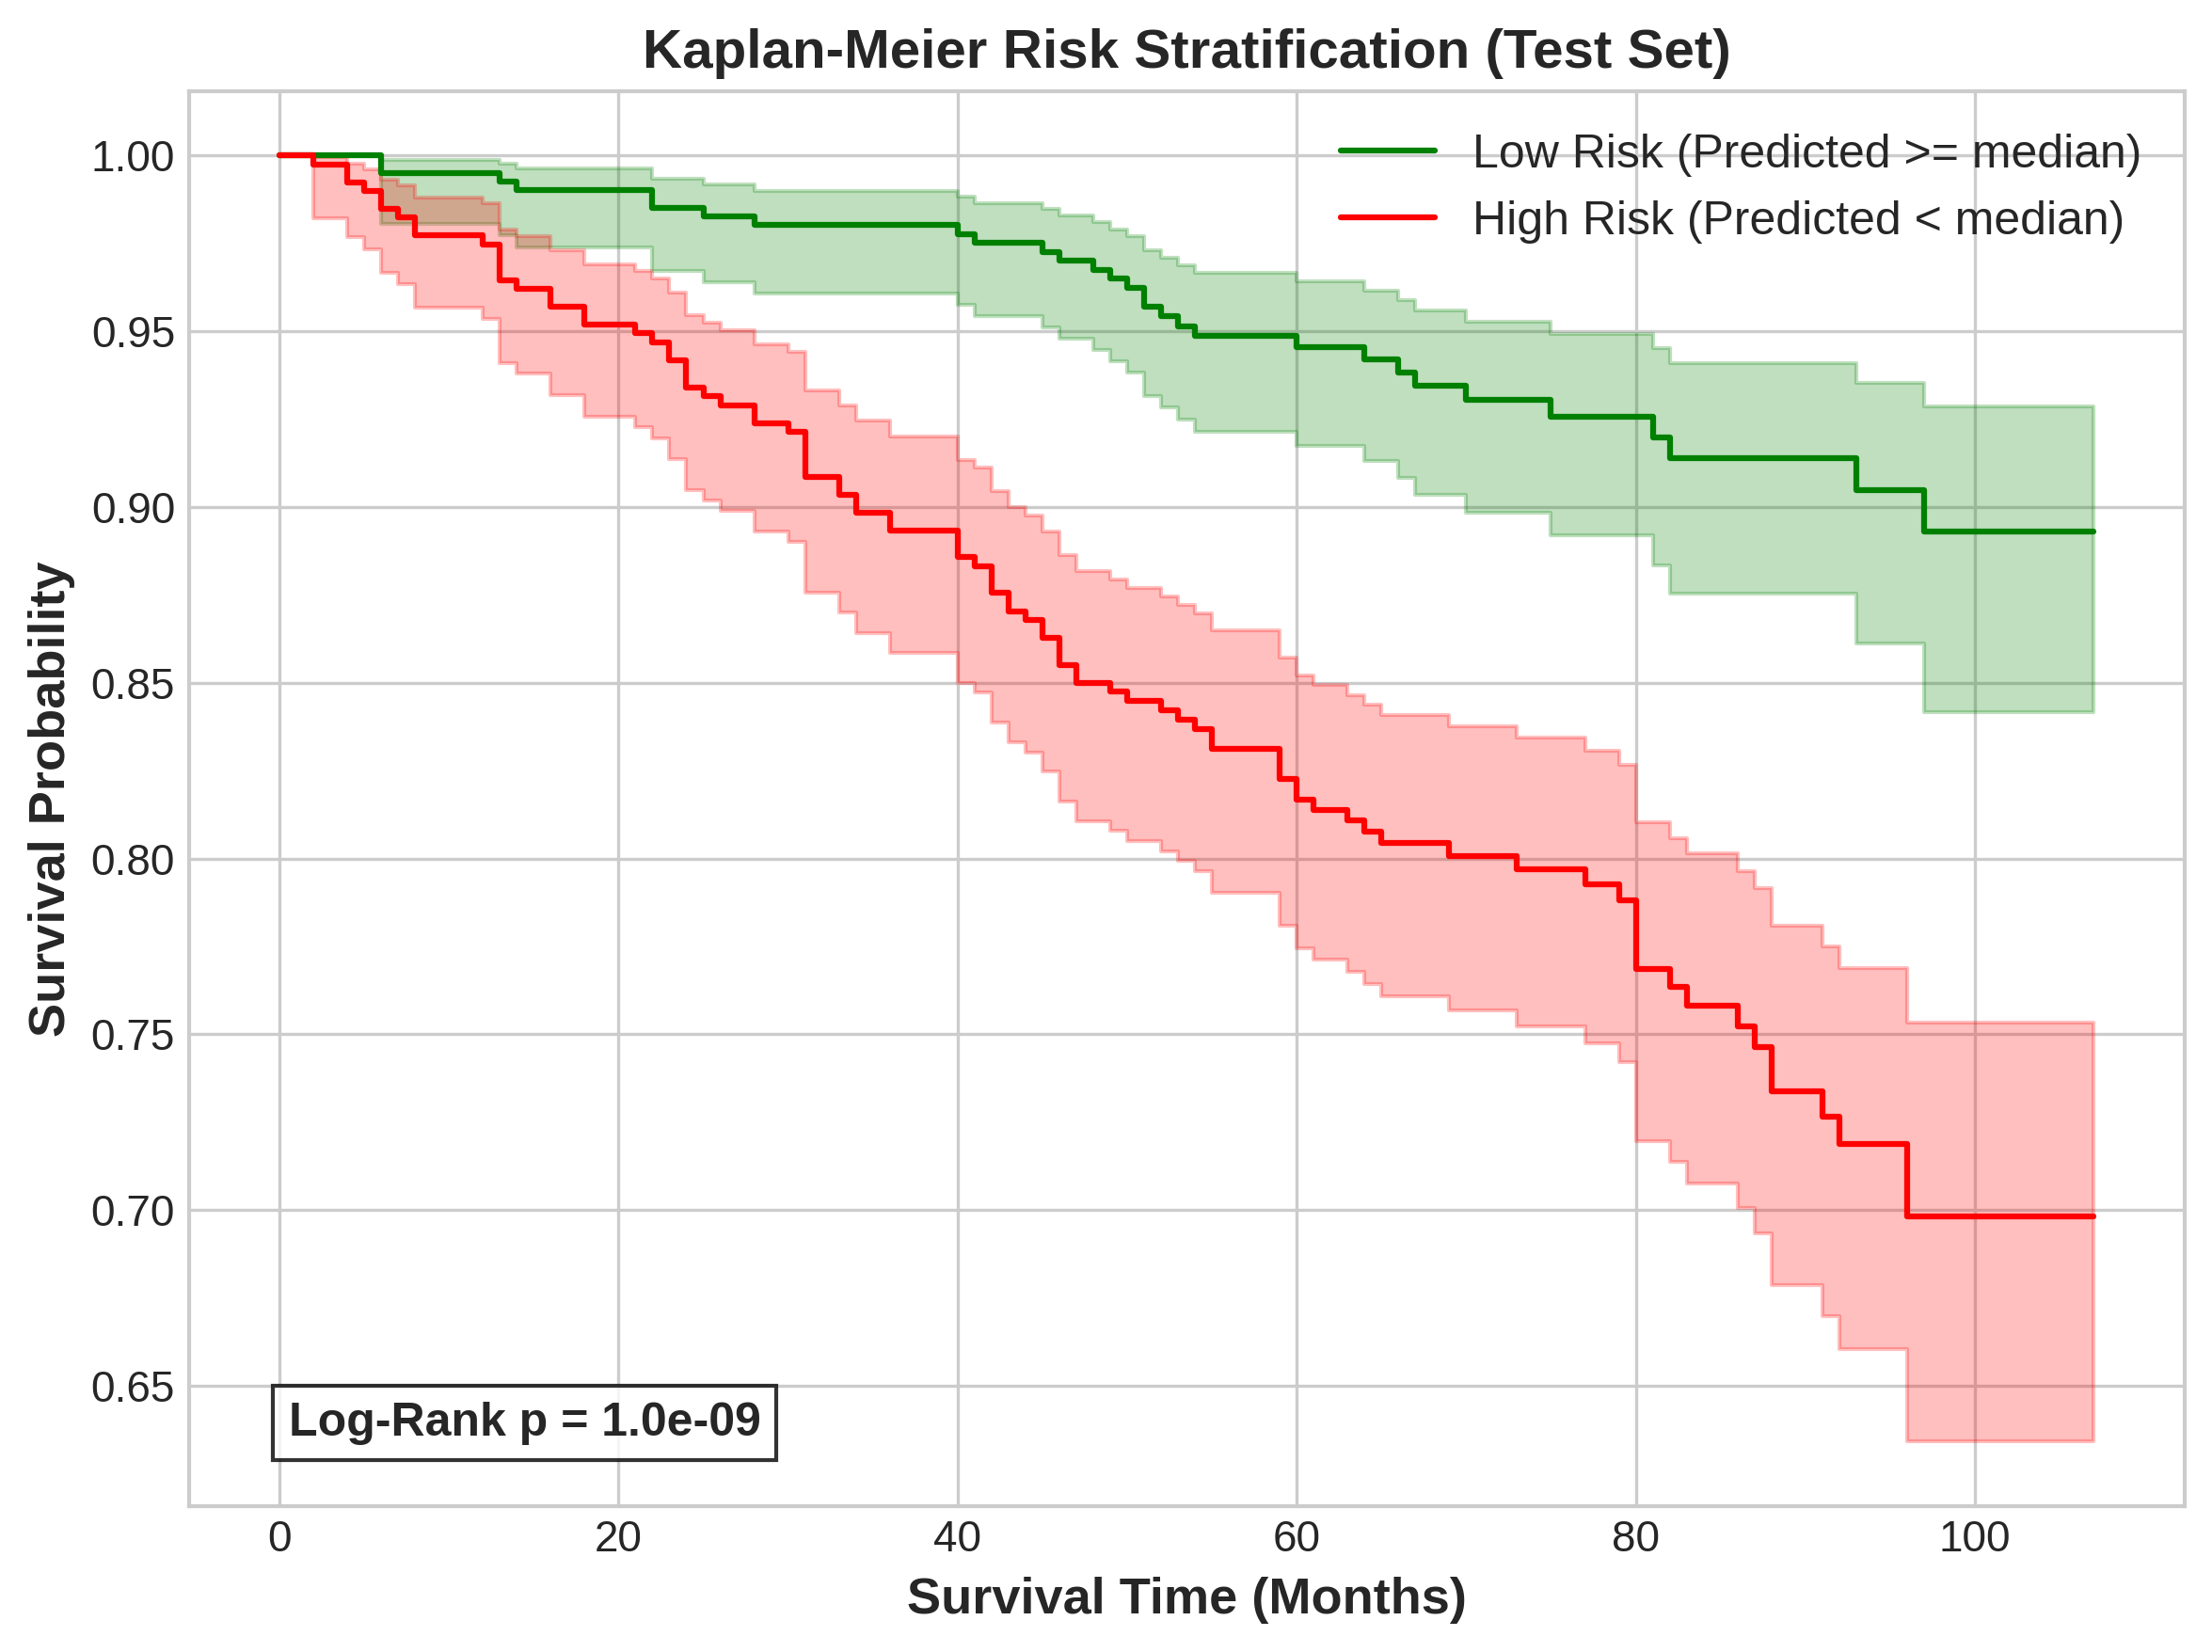
\includegraphics[width=0.72\textwidth]{figs/SEER_AFT_KM_Stratification.png}
\caption{Kaplan--Meier survival stratification on the SEER survival test partition using groups defined by the training-set median predicted survival from the penalised Weibull AFT model.}\label{fig:km}
\end{figure}

\section{Discussion}\label{sec:disc}
\subsection{Leakage, Architecture Adaptation, and Benchmark Comparison}\label{sec:leakage-architecture-adaptatio}
Tadj et al.\ audited pre-split oversampling contamination using row-hash checks on static splits and penalised Weibull models~\cite{tadj2026}. TRUST-BC targets a different class of leakage---parametric and covariance leakage in repeated cross-validation---by ensuring that scaling parameters $(\hat{\mu},\hat{\sigma})$ and subspace bases $W_d$ never cross evaluation partitions.

The architecture-matched contrast (Table~\ref{tab:leak}) is the central empirical finding of this revision: global scaling and PCA produced negligible optimism in all three cohorts. This is plausible, because the only information that leaks is unsupervised (feature means, variances and principal axes), which is estimated almost identically from 80\% or 100\% of the development data when samples are moderately large and the transforms do not use the outcome. It contrasts sharply with outcome-dependent leakage such as pre-split oversampling, which Tadj et al.\ showed can inflate AUROC from 0.715 to 0.998~\cite{tadj2026}. Our earlier interpretation, that non-equivalence with the leaky baseline in Coimbra and SEER reflected ``leakage-driven optimism'', is not supported: in both cohorts the leakage-free Unified pipeline performed at least as well as the leaky baseline, and the difference arose from adaptive RF feature selection. The practical conclusion is that leakage risk depends on the type of leakage and on the data, and must be measured with a design that isolates it; a blanket assumption that any preprocessing leakage materially inflates every estimate is as unsound as ignoring leakage altogether. Per-cohort auditing with an architecture-matched comparator, as implemented here, distinguishes these situations empirically.

The internal selector chose PCA in 94\% of WBCD folds and RF in 92\% of Coimbra and \seerRFpct\% of SEER folds, indicating that automated architecture switching responds to data geometry: strongly collinear continuous cytomorphometric features favour PCA compression, whereas discrete staging variables and non-linear metabolic markers favour impurity-based selection. In Coimbra, the Unified pipeline (71.35\%) was slightly below the Nested RF ablation (72.37\%) because, in 4 of 50 folds, the inner search chose PCA owing to validation noise, with outer-fold drops (e.g., 68.4\% vs 89.5\%). This ``cost of flexibility'' is expected when selector search is performed in very small samples ($n=116$).

The SEER survival C-index (0.722) was similar to the cross-validated classification AUROC (\seerUniAUC). This alignment suggests that the discrimination observed in the classification branch is not solely an artefact of the binary 5-year cut-off. Because the survival and classification partitions were drawn independently from overlapping source data with different eligibility criteria, the two estimates are complementary rather than fully independent confirmations.

\begin{table}[htbp]
\centering\footnotesize
\setlength{\tabcolsep}{3pt}
\caption{Methodological and quantitative comparison of representative clinical machine learning studies and reviews.}\label{tab:lit}
\begin{tabularx}{\textwidth}{@{}P{1.9cm}P{1.5cm}P{1.6cm}P{1.6cm}P{2.1cm}YP{1.3cm}P{1.4cm}@{}}
\toprule
\textbf{Study} & \textbf{Cohort(s)} & \textbf{Algorithm} & \textbf{CV scheme} & \textbf{Reported metric} & \textbf{Leakage control} & \textbf{Conformal UQ} & \textbf{Calibration}\\
\midrule
Street et al.\ (1993)~\cite{street1993} & WBCD & Linear programming & 10-fold (unnested) & Accuracy $\approx$97.0\% & None & No & No\\
Asri et al.\ (2016)~\cite{asri2016} & WBCD & SVM, NB, C4.5 & 10-fold (unnested) & Accuracy $\approx$97.13\% & None & No & No\\
Patr\'icio et al.\ (2018)~\cite{patricio2018} & Coimbra & SVM, RF & Single split (70/30) & AUROC $\approx$0.87--0.91 & None & No & No\\
Liu et al.\ (2025)~\cite{liu2025} & CVD EHRs (21 studies) & Review and meta-analysis & Not fully reported & Pooled RF AUROC 0.865 & Not evaluated & Not assessed & Not fully reported\\
Tadj et al.\ (2026)~\cite{tadj2026} & SEER ($N=4{,}024$) & SVM; Weibull AFT & Single split (80/20) & AUROC 0.998$\rightarrow$0.715 & Pre-split oversampling (row-hash audit) & No & No\\
TRUST-BC (present study) & WBCD, Coimbra, SEER & Unified LR--SVC & Repeated nested CV & Accuracy 97.08\%, 71.35\%; SEER AUROC \seerUniAUC & Parametric \& covariance (architecture-matched contrast) & Yes (95\%) & Yes (ECE, Brier, CITL, DCA)\\
\bottomrule
\end{tabularx}
\end{table}

\subsection{Conformal Uncertainty Quantification for Clinical Decision Support}\label{sec:conformal-uncertainty-quantifi}
Split conformal prediction converts model probabilities into prediction sets with a distribution-free marginal coverage guarantee of at least 95\% under exchangeability~\cite{angelopoulos2021}. Ambiguous-set rates tracked cohort discriminability: WBCD produced singleton sets for 97.40\% of predictions, Coimbra for 27.70\% and SEER for \seerConfSingle\%. The substantial ambiguous fraction in SEER (\seerConfAmb\%) reflects the intrinsic uncertainty of predicting 5-year mortality from staging and demographic covariates alone. Rather than silently returning an overconfident probability, the framework routes these cases to expert review. However, the SEER analysis also shows the limits of marginal coverage: deaths were covered in only 69.9\% of cases compared with 99.4\% of survivors, and coverage ranged from \seerCovRange{} across race and age subgroups. Class-conditional (Mondrian) conformal prediction, which calibrates each outcome class separately, would be required if equal coverage of deaths is a clinical requirement.

\subsection{Clinical Implementation as a Decision Support System}\label{sec:clinical-implementation-as-a-d}
In a prospective workflow, TRUST-BC would serve as an auxiliary clinical decision support system rather than an autonomous triage tool. Historical registry cohorts (SEER 2006--2010) lack exposure to contemporary systemic and targeted therapies, so the framework aims to assist rather than dictate management.
\begin{enumerate}
\item \textbf{Higher-confidence predictions (singleton sets):} patients receiving singleton sets ($|\mathcal{C}|=1$; 97.40\% of WBCD, 27.70\% of Coimbra and \seerConfSingle\% of SEER cases) could be presented to the clinician as higher-confidence predictions. The conformal guarantee is marginal: on average over exchangeable patients, sets contain the true label with probability at least 95\%. It does not provide a per-patient or per-subgroup error bound, and singleton predictions still require clinician confirmation before any management decision.
\item \textbf{Clinical escalation (ambiguous sets):} patients with $|\mathcal{C}|=2$, the majority in non-invasive metabolic screening such as the Coimbra panel, are flagged for further clinical evaluation rather than automated invasive procedures. Secondary evaluation is non-prescriptive and guided by clinical context (age, examination findings such as palpable masses or mastalgia, family history) to determine the next step, such as diagnostic mammography, breast ultrasound or targeted follow-up.
\end{enumerate}
\paragraph{Input data and user expertise.} The pipeline requires complete predictor values and was developed only on complete cases. If a predictor is missing or outside the range observed in the development data, the prediction should not be produced automatically; the case should be flagged for manual review, and imputation would require separate validation. Out-of-range values can be detected by comparing each input with the training minimum and maximum, which the released code reports. Users must supply correctly coded predictors (for example, AJCC 6th-edition T and N categories for SEER) and need clinical expertise to interpret probabilities and prediction sets; the model is not intended for use by patients or without clinician oversight.

\subsection{Comparison with Established Clinical Prognostic Systems}\label{sec:comparison-with-established-cl}
Established instruments such as the Nottingham Prognostic Index~\cite{galea1992}, PREDICT~\cite{candido2017} and the AJCC staging system~\cite{giuliano2017} are based on pre-defined risk scores derived from large populations and, in the case of PREDICT, include treatment effects and have been externally validated. TRUST-BC does not replace these tools; its models were internally validated only and, for SEER, were poorly calibrated in the large. Its contribution is to add conformal uncertainty and a systematic calibration audit to the development workflow.

\subsection{Limitations}\label{sec:limitations}
\begin{enumerate}[leftmargin=*]
\item \textbf{Calibration comparison asymmetry:} XGBoost and LightGBM probabilities were not recalibrated, whereas the LR--SVC pipelines include Platt scaling. This mainly affects Brier score and ECE; AUROC is invariant to monotonic recalibration, but threshold-dependent accuracy is not. Future extensions should recalibrate all baselines consistently.
\item \textbf{Historical, small benchmark cohorts:} WBCD ($n=569$, collected before 1993) and Coimbra ($n=116$, 2009--2013) are small; Coimbra does not meet the Riley minimum sample size (381) and its EPV is 5.8.
\item \textbf{Case--control design of Coimbra:} comparing women with breast cancer with healthy controls overstates discrimination and distorts calibration relative to a screening population with lower prevalence and more heterogeneous non-cases, so Coimbra results are not evidence of screening performance.
\item \textbf{Omission of deep tabular baselines:} TabNet and FT-Transformer were omitted because small samples favour regularised linear ensembles and gradient-boosted trees~\cite{shwartz2022}.
\item \textbf{Exclusion of censored patients:} excluding patients censored before 60 months avoids labelling them as survivors, but if censoring is associated with prognosis the remaining cohort is selected and 5-year mortality and calibration may be biased. Inverse probability of censoring weighting~\cite{vock2016} or direct use of survival models would address this; the survival branch partly does so.
\item \textbf{SEER label correction and partial re-analysis:} the v1.0 analysis labelled 158 deaths after month 60 as 5-year events. The corrected re-analysis reproduced the v1.0 fold-level results exactly under the original label (Supplementary Section~S8) but re-ran only the scikit-learn pipelines; the gradient boosting baselines were not re-run for the corrected endpoint, and Shapley values were estimated by permutation sampling rather than Kernel SHAP.
\item \textbf{SEER overprediction:} balanced class weighting produced calibration-in-the-large of about $-1.0$ (mean predicted risk \seerMeanPred\% vs 14.0\% observed). Probabilities should be recalibrated before any use as absolute risks.
\item \textbf{Retrospective registry scope and population:} the SEER extraction lacks treatment regimens, HER2 status and comorbidity, is restricted to node-positive women aged 30--69 years diagnosed in 2006--2010, and contains all-cause rather than breast-cancer-specific mortality.
\item \textbf{Small evaluation samples:} the lockboxes contain 32 (WBCD), 10 (Coimbra) and 69 (SEER) events, below the commonly recommended minimum of 100 events~\cite{collins2016,riley2021val}. The WBCD calibration slope and the Coimbra coverage are therefore highly uncertain; the cross-validated estimates (Table~\ref{tab:bench}) are the more reliable summaries.
\item \textbf{Marginal conformal coverage and exchangeability:} coverage holds on average and not within outcome classes or subgroups (SEER deaths 69.9\%). Guarantees also require exchangeability, which may fail under temporal or geographic shift. Hyperparameters of the conformal model were selected on the whole development set, which includes the conformal test subsets, so development-set coverage may be slightly optimistic; the lockbox coverage is not affected.
\item \textbf{Fixed dimensionality heuristic:} $d$ was set by a pre-specified heuristic rather than tuned; Figure~\ref{fig:dim} is a post hoc sensitivity analysis.
\item \textbf{Duplicate and temporal leakage audit scope:} exact sample-hash overlap was checked, but no near-duplicate search or temporal leakage audit was performed.
\item \textbf{No external or prospective validation:} utility was evaluated by in-silico DCA only, and models were not evaluated in other healthcare systems. External validation, for example in METABRIC, is the most important next step and would be an independent contribution.
\item \textbf{Survival C-index interval:} the CI was obtained from a re-implementation of the Weibull model that reproduced the point estimate to within 0.002, not from the original fitted object.
\item \textbf{Gradient boosting with minimal hyperparameter search:} the grids (eight combinations per library) were deliberately narrow for computational feasibility; the failure of these baselines to outperform the Unified pipeline reflects the tuning budget, not a limitation of gradient boosting.
\item \textbf{Author self-assessment of bias:} the PROBAST+AI assessment (Supplementary Table~S2) was performed by the authors, not by independent reviewers.
\item \textbf{Fairness analysis scope:} subgroup analyses were limited to race and age in SEER, with small numbers of events among Black and Other-race patients; no sociodemographic variables are available in WBCD.
\end{enumerate}

\section{Conclusion}\label{sec:conclusion}
TRUST-BC is a multicohort benchmark and auditing template that jointly assesses preprocessing leakage, fixed-horizon labelling, calibration and predictive uncertainty. The leakage-free Unified pipeline obtained 97.08\% accuracy on WBCD, 71.35\% on Coimbra and an AUROC of \seerUniAUC{} for 5-year all-cause mortality in SEER. An architecture-matched comparison showed that global scaling/PCA leakage produced negligible optimism in all three cohorts, and that non-equivalence with the leaky baseline in Coimbra and SEER reflected adaptive feature selection. The audit instead identified other, larger problems: horizon mislabelling in the registry cohort (158 of 616 deaths), marked overprediction of SEER risk after class weighting, and conformal under-coverage of deaths despite nominal marginal coverage. An independent Weibull AFT survival branch attained a C-index of 0.722 (approximate 95\% CI 0.675--0.771) with significant risk separation. These findings illustrate why leakage, labelling, calibration and uncertainty should be audited per cohort rather than assumed. Future work should validate the framework in geographically distinct external registries, recalibrate probabilities, use class-conditional conformal prediction, and extend audits to near-duplicate, site-specific and temporal leakage.

\section{Future Work}\label{sec:future-work}
Metabolic panels such as Coimbra rely on general metabolic markers (e.g., glucose, insulin, resistin). Future iterations should incorporate breast-cancer-specific biomarkers and circulating tumour markers in prospectively collected cohorts, which is expected to improve discriminability and reduce the proportion of ambiguous prediction sets in non-invasive screening.

\section*{Declarations}\label{sec:declarations}
\small
\noindent\textbf{Ethics approval and consent to participate:} Ethical review was not required because all analyses used publicly available, fully de-identified retrospective datasets.

\noindent\textbf{Consent for publication:} Not applicable.

\noindent\textbf{Protocol and registration:} A formal study protocol was not prepared and the study was not registered. The analysis plan (partitioning scheme, primary metrics, hypothesis-testing family and TOST margins) was fixed in the analysis code before model development and is available in the repository history.

\noindent\textbf{Patient and public involvement:} Patients and members of the public were not involved in the design, conduct, reporting, interpretation, or dissemination of this study.

\noindent\textbf{Reporting guidelines:} The completed TRIPOD+AI and TRIPOD+AI for Abstracts checklists are provided in Supplementary Table~S1. An author self-assessment against PROBAST+AI is provided in Supplementary Table~S2.

\noindent\textbf{Data and code availability:} Source code, split manifests, fold-level scores, out-of-fold and lockbox predictions, supplementary analyses and evaluation logs are available at \url{https://github.com/mohammdreza-ui/TRUST-BC-Multicohort-Benchmark} (release v1.1, MIT licence). The re-analysis scripts in \texttt{scripts/} regenerate all revised SEER results from the public SEER file. WBCD and Coimbra are available from the UCI Machine Learning Repository~\cite{uci}; the SEER research extraction is available from public benchmark archives~\cite{namdari2019}.

\noindent\textbf{Software and computational environment:} The v1.0 analyses were implemented in Python 3.10 with scikit-learn 1.6.1~\cite{sklearn}, XGBoost 3.4.1~\cite{xgboost}, LightGBM 4.6.0~\cite{lightgbm}, SHAP 0.52.0~\cite{lundberg2017}, NumPy 2.1.3, SciPy 1.16.3 and lifelines 0.30.3. The v1.1 SEER re-analysis used scikit-learn 1.8.0, NumPy 2.4.4, SciPy 1.17.1 and pandas 3.0.2 on a single CPU; under the original label it reproduced all v1.0 fold-level scores of the four scikit-learn pipelines exactly (Supplementary Section~S8). Machine-level telemetry was not logged for the v1.0 run.

\noindent\textbf{Declaration of Generative AI and AI-Assisted Technologies in the Writing Process:} During the preparation of this work, the authors used OpenAI's ChatGPT and Anthropic's Claude to grammatically edit the manuscript and debug the Python scripts. After using these tools, the authors reviewed and edited the content as needed and take full responsibility for the accuracy of the content.

\noindent\textbf{Funding:} This research received no specific grant from any funding agency in the public, commercial, or not-for-profit sectors.

\noindent\textbf{Conflict of interest:} The authors declare no competing financial interests or personal relationships that could have influenced this work.

\normalsize
\bibliographystyle{unsrtnat}
\bibliography{refs}
\end{document}
